%
%
%
%
\section{Steady State Flow Analysis}
\label{rt27_steady.sec}
\headb{Transonic Turbine Stage}{Steady state flow}
%
%
 The analysis of the steady-state flow-field for
 the coupled NGV-rotor configuration is presented in this section.
 The flow is assumed to be fully turbulent
 and the high Reynolds number version of the Spallart-Allmaras
 \citeyear{Spalart:1} turbulence model
 is used together with a slip boundary condition on the solid walls. The
 wall shear stresses are evaluated using a generalized law of the wall
 as the one reported by White \citeyear{White:1}.
 Apart from predicting midspan pressure more accurately,
 3D calculations provide us with hub to tip
 distribution of the dependent variables
 and take the tip losses into account.
 When the air is turned through a row of axial blades,
 the flow far from the end walls,
 hub or casing, may often be considered as 2D.
 However near the end walls, the inlet boundary layer flow contains
 span-wise velocity gradients, and transverse velocities
 are produced once it is turned.
 The 2D flow is termed the {\em primary} flow
 and the 3D effects near the end walls are called {\em secondary}
 flows.
 Furthermore a turbomachinery rotor blade must have a small but finite clearance
 relative to its surrounding casing. The clearance, as in the case of rotor RT27a,
 is typically $1\%$ of the blade's span. However, the flow which leaks through
 this small gap has a surprisingly large effect on the aerodynamics of the machine
 especially when the blade is relatively short.
 In order to predict secondary flow effects and to take into account
 tip-leakages, the hub and tip sections must be treated as solid walls
 and a tip clearance must be included in the computational mesh.
%
%
%
\subsection{Computational mesh}
\label{rt27_mesh.subsec}
%
\begin{figure}
~\vspace{-30mm}\\
 \begin{center}
  \begin{tabular}{c}
    \subfigure[3D view]
       {\centerline{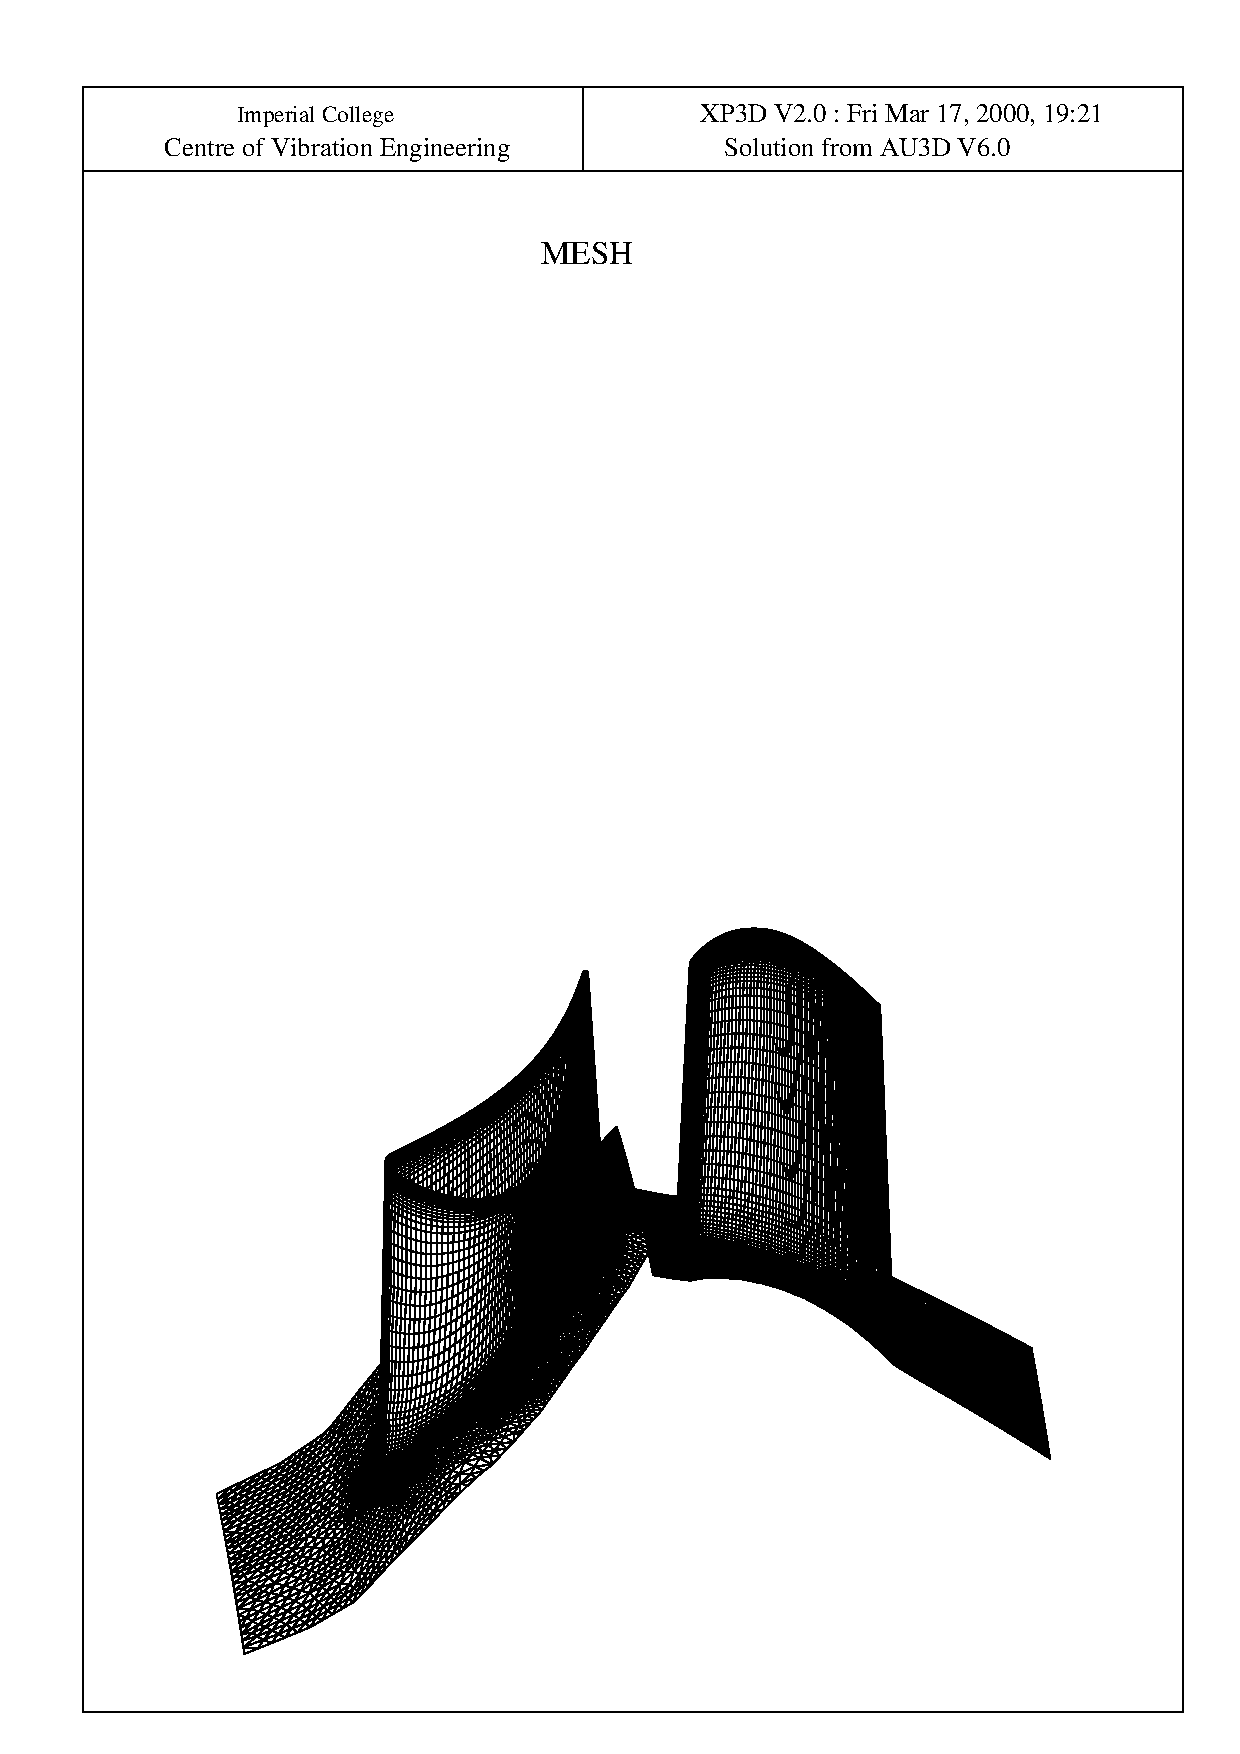
\includegraphics[width=140mm,clip=t]{CHAP_RT27/FIGURE/mesh3d_1.pdf}}}
        \vspace{-5mm}\\
    \subfigure[Meridional view]
       {\centerline{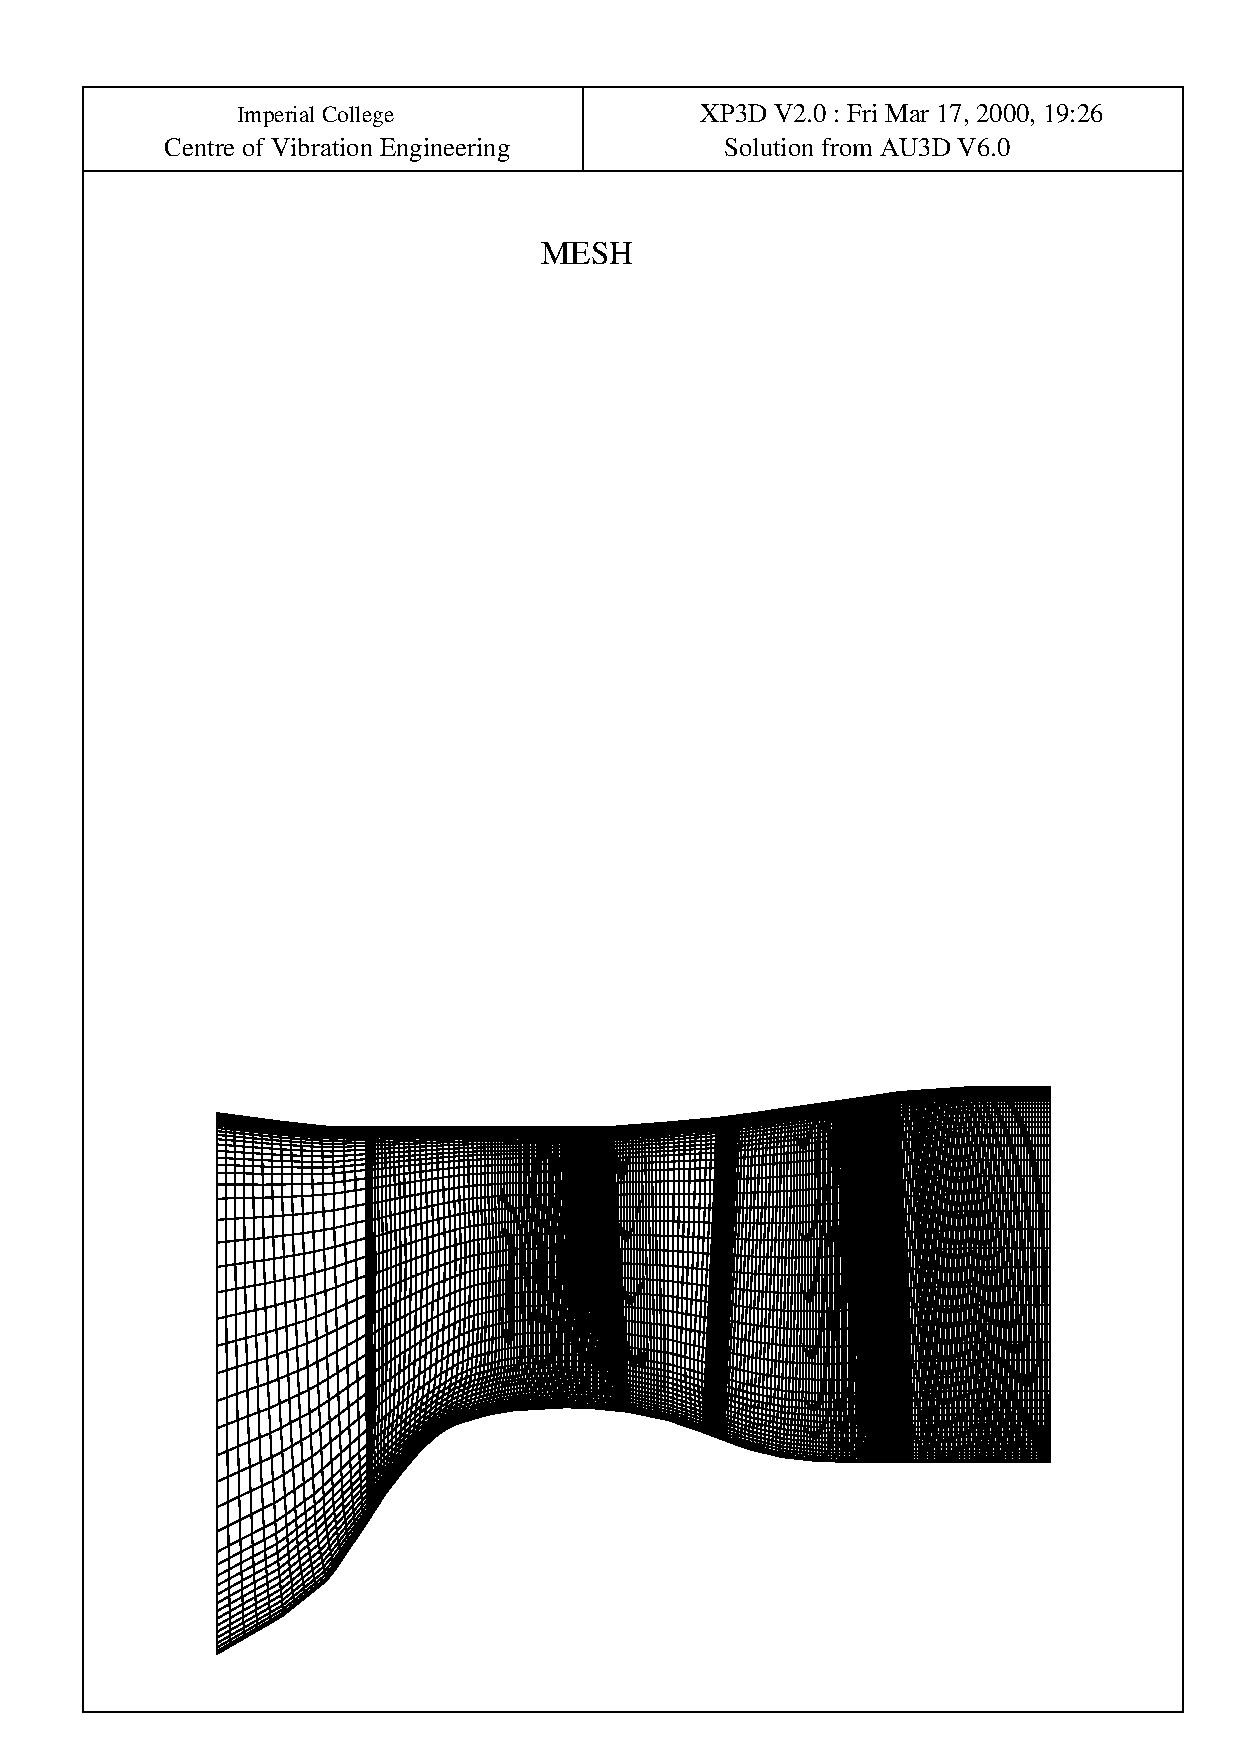
\includegraphics[width=140mm,clip=t]{CHAP_RT27/FIGURE/mesh3d_3.pdf}}}
  \end{tabular}
 \end{center}
 \vspace{-8mm}
 \caption{Computational mesh of RT27a turbine stage (564,660 points)}
 \label{rt27_mesh1.fig}
\end{figure}
%
 The computational meshes for the NGV and rotor passages were generated
 independently using the LEVMAP mesh generator described in chapter \ref{mesh.chap}.
 These two meshes were then assembled together for a coupled
 NGV-rotor steady-state calculation.
 The NGV outflow and rotor inflow are treated
 as two separate boundaries and they are responsible for the interaction
 between the two domains via a mixing layer process (Dawes \citeyearNP{Dawes:4},
 Denton \citeyearNP{Denton:1}).
 A 3D view of the grid is shown in Fig. \ref{rt27_mesh1.fig}a
 while Fig. \ref{rt27_mesh1.fig}b shows
 a meridional view of the blade surfaces together with one periodic boundary.
 The points in the radial direction are clustered towards the end walls
 because of the strong secondary flow expected in these regions. Also,
 additional grid radial-levels are used in the rotor tip-gap region
 to capture the tip leakage effects.
%
\begin{figure}[ht]
 \begin{center}
  \begin{tabular}{cc}
    \subfigure[Tip-gap radial mesh]
       {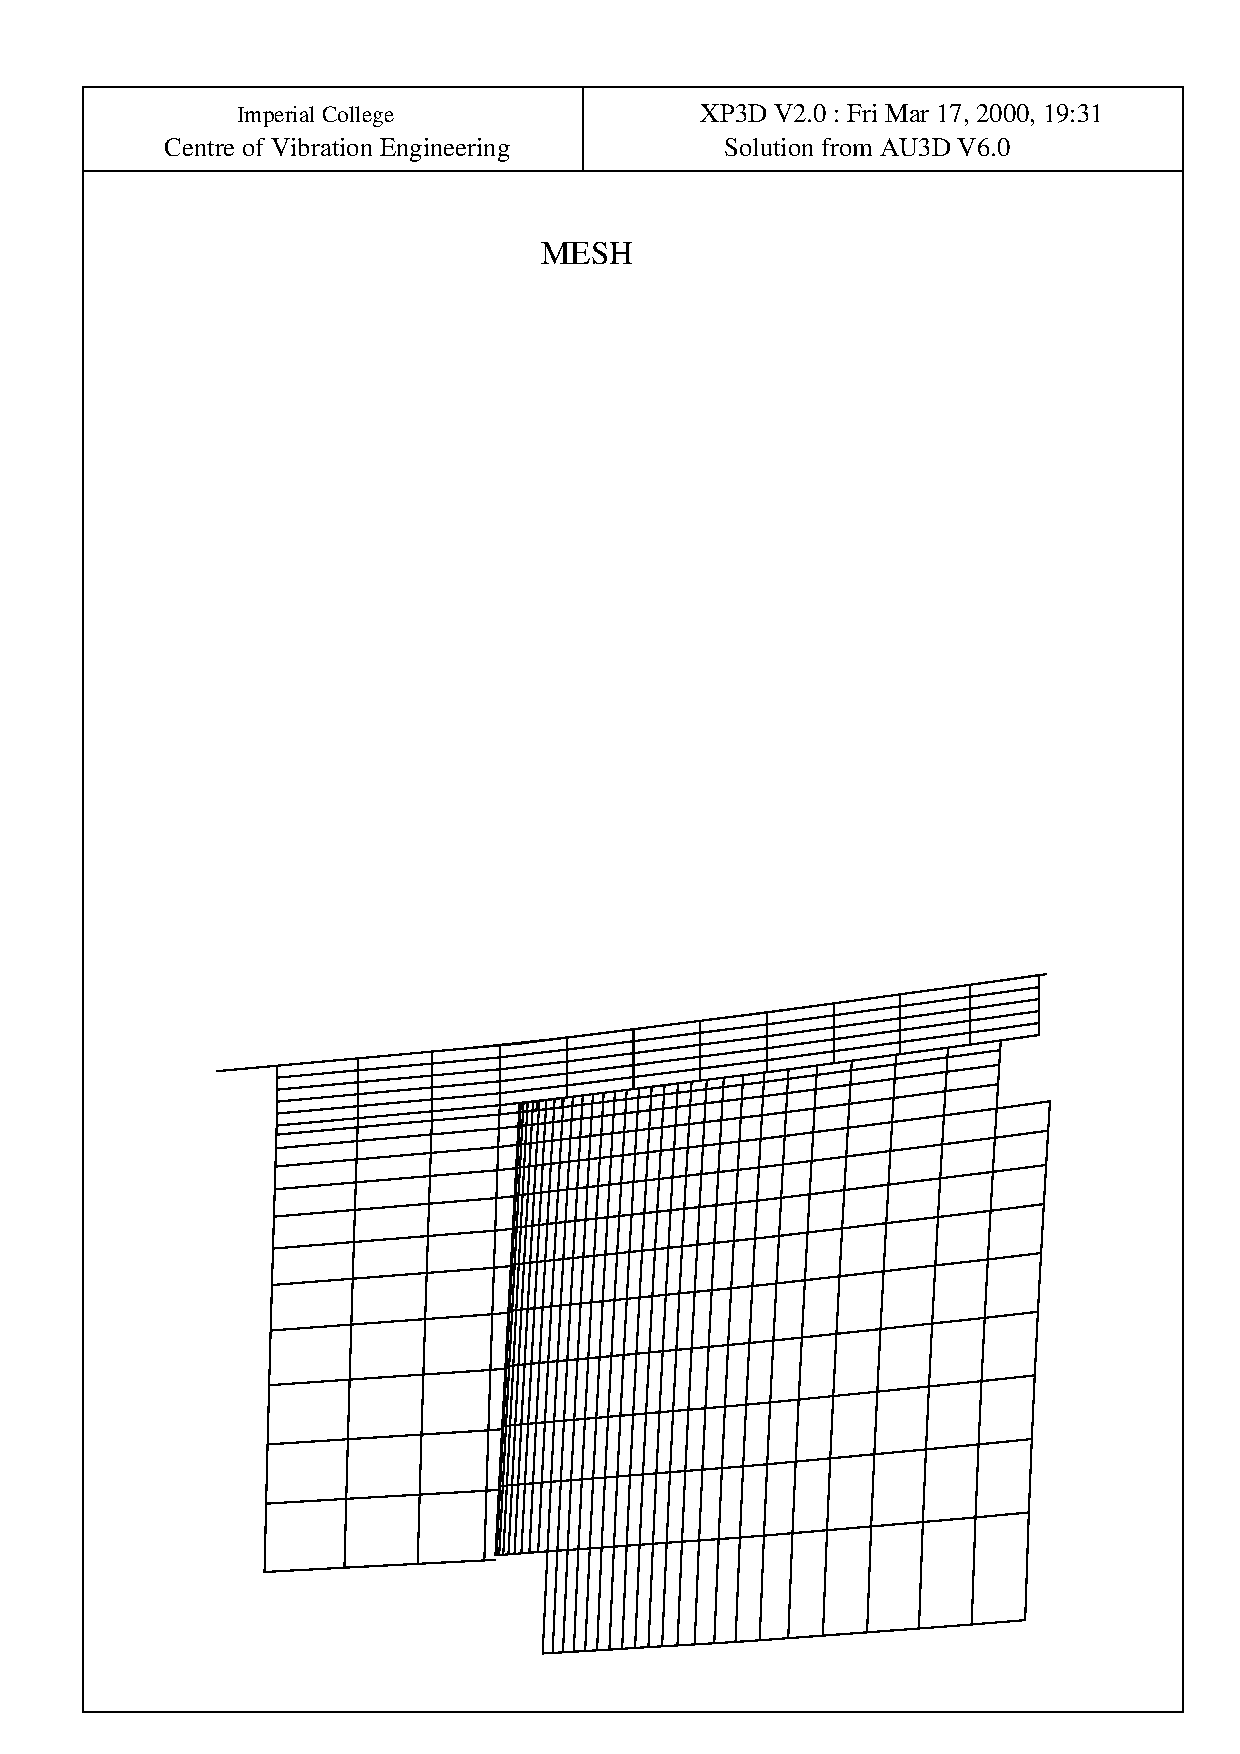
\includegraphics[width=70mm,clip=t]{CHAP_RT27/FIGURE/mesh3d_4.pdf}}
        &
    \subfigure[Tip-section]
       {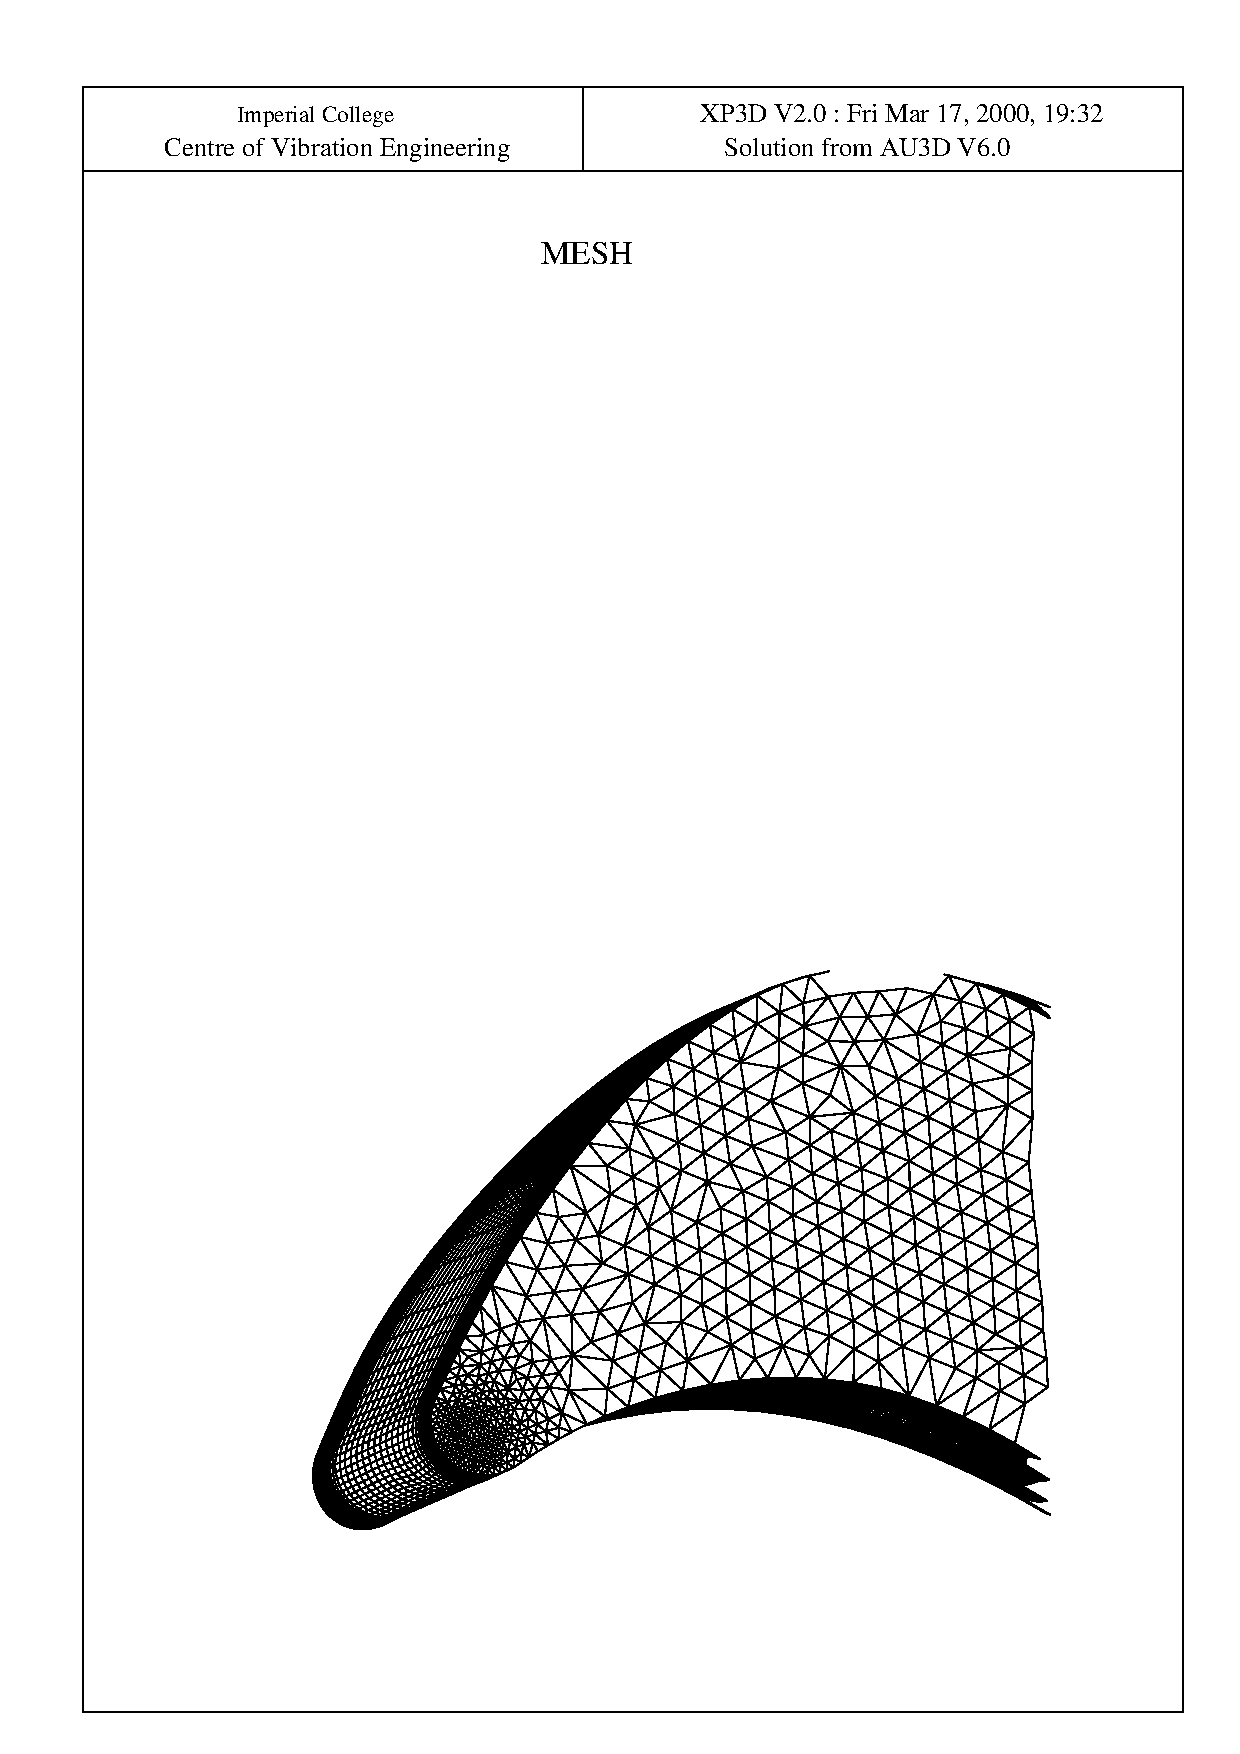
\includegraphics[width=70mm,clip=t]{CHAP_RT27/FIGURE/mesh3d_5.pdf}}
  \end{tabular}
 \end{center}
 \vspace{-8mm}
 \caption{Computational mesh at tip end wall of RT27a rotor blade}
 \label{rt27_mesh2.fig}
\end{figure}
%
 Both grids have 48 points in the radial direction, the
 locations at the NGV-outlet and rotor-inlet being identical
 (Fig. \ref{rt27_mesh1.fig}b).
 As shown in Fig. \ref{rt27_mesh2.fig}a, 42 of the radial grid levels,
 define the rotor geometry while the remaining six are positioned
 in the tip-gap region.
 Fig. \ref{rt27_mesh2.fig}b shows the triangulation of the
 rotor tip section.

 Both the NGV and the rotor boundary layer regions are discretised by
 a twelve-layer of O-type mesh formed by hexahedra elements.
 Such a resolution is sufficient for a viscous computation
 which uses the law of the wall to evaluate the wall shear stresses.

 Fig. \ref{rt27_mesh3.fig} shows the mid-height radial section
 of the computational mesh.
 The NGV grid contains 4,717 points per radial level which yields a total
 of 226,416 points.
 The inclusion of the NGV passage in the steady-state computation
 is mainly justified by the need of (i) predicting a correct steady-state
 inlet conditions for the rotor passage and (ii) the evaluation of the
 spatial non-uniformities at the NGV-outlet.
 For these reason the NGV-grid is refined in the trailing-edge
 and outflow regions.
%
\begin{figure}[ht]
 \centerline{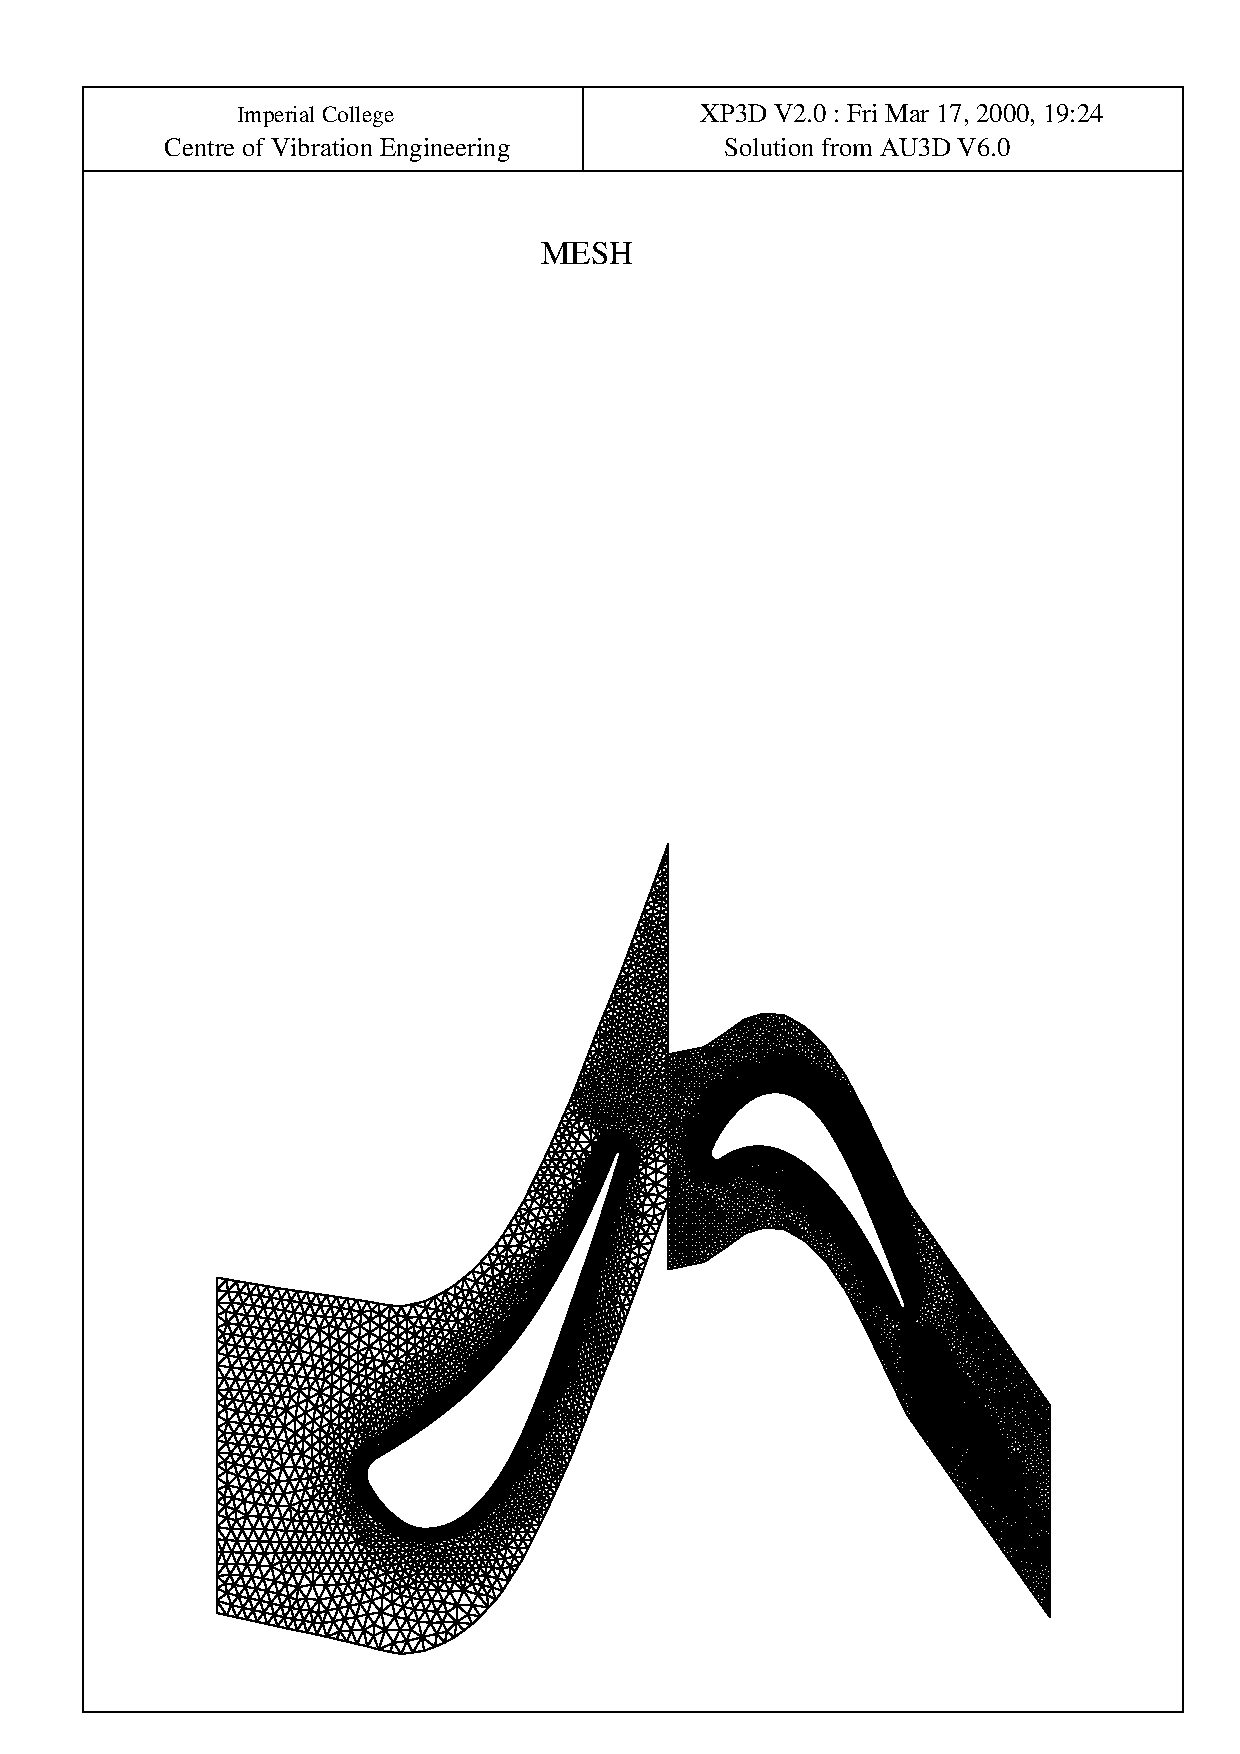
\includegraphics[width=140mm,clip=t]{CHAP_RT27/FIGURE/mesh3d_2.pdf}}
 \caption{Computational mesh at mid-height section of RT27a turbine stage}
 \label{rt27_mesh3.fig}
\end{figure}
%
 The rotor grid contains 338,244 points distributed in the following way:
 each one of the six radial section in the tip-clearance region
 contains 7,850 points while each one of the remaining 42 sections
 contains 6,932 points. The number of points positioned in the
 rotor tip section of Fig. \ref{rt27_mesh2.fig}b is 918.
%
\begin{table}
\vspace{5mm}
\begin{center}
\begin{tabular}{|l|l|}\hline\hline
 Periodic boundary (axial direction) & 126\\ \hline
 Inflow boundary (tangential direction)& 41\\ \hline
 Outflow boundary (tangential direction)& 43\\ \hline
 Blade suction side (axial direction)& 110\\ \hline
 Blade pressure side (axial direction)& 108\\ \hline
\hline
\end{tabular}
\end{center}
\caption{Number of point on domain boundaries of RT27a rotor blade}
\label{rotor_mesh.tab}
\end{table}
%
 Table \ref{rotor_mesh.tab} lists the number of points in each boundary
 of a rotor radial section.

 The tip clearance grid is relatively coarse since the main interest
 is not to predict accurately the structure of the tip-leakage flow,
 but only to take into account its main effect on the
 hub-to-tip pressure distribution.
 Since the main parameters which can affect the pressure distribution
 towards the tip are the size of the clearance and the
 pressure jump across the blade,
 the tip-grid of Fig. \ref{rt27_mesh2.fig}
 is considered to be sufficient for the purposes of the current analysis.
%
%
%
\subsection{Boundary conditions and computational details}
\label{rt27_boundary.subsec}
%
 The boundary conditions, together with the rotor rotational speed,
 specify at which point in the turbine stage characteristic the calculation
 is performed. The nominal design condition has been chosen for
 this numerical analysis. The rotor rotational speed is the one
 reported in table \ref{rt27.tab}. The NGV inlet conditions are the
 following: constant stagnation
 pressure ($p\sm{01}$ in table \ref{rt27.tab}), constant
 stagnation temperature ($T\sm{01}$ in table \ref{rt27.tab}),
 flow direction without tangential component ($\alpha\sm{x\theta} = 0$) and
 flow angle in the $x-r$ plane reported in Fig. \ref{bcond.fig}a.
 The final boundary condition is applied at the rotor outlet where
 the static pressure distribution of Fig \ref{bcond.fig}b is specified.
 A sequence of three agglomerated grid levels were generated for both the
 NGV and the rotor domains so that a 4-grid W-cycle algorithm was used
 for the steady state computations.
 Starting from free-stream conditions the computation took around 300
 multigrid cycles to converge. The calculation was
 performed on a 500 MHz DEC Alpha machine where the 300 multigrid cycles
 were completed in about 8 hours.
 The average $y+$, which indicates the the resolution of the viscous body fitted
 O-grid, was of around 150 while the maximum was $\approx 500$.
 Both these values are within the logaritmic part of the turbulent
 boundary layer thus justifying the grid-resolution in this region.
%
\begin{figure}[ht]
 \begin{center}
  \begin{tabular}{cc}
    \hspace{-10mm}
    \subfigure[NGV inlet flow angle in the $x-r$ plane]
       {\includegraphics[height=60mm,clip=t]{CHAP_RT27/FIGURE/alphaxr.pdf}}
        &
    \subfigure[Rotor outlet static pressure]
       {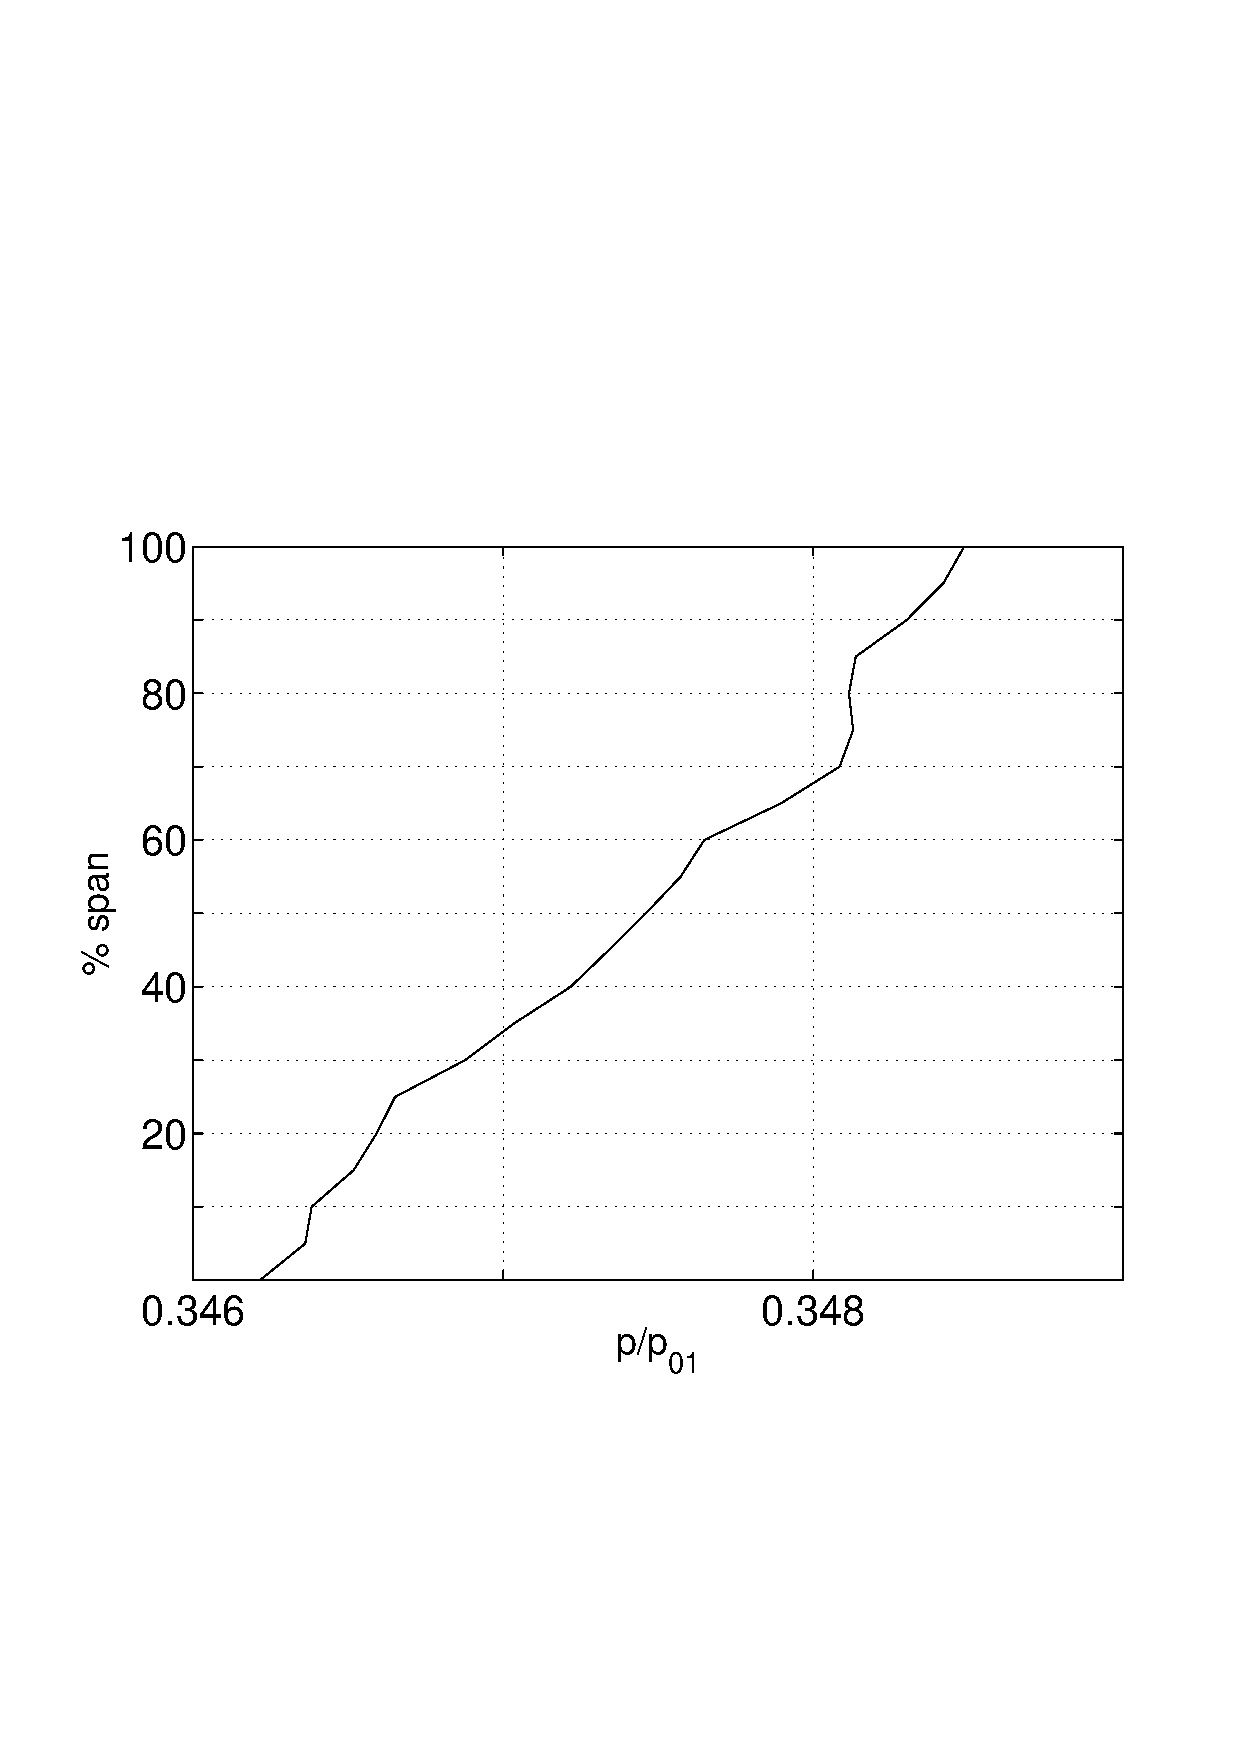
\includegraphics[height=60mm,clip=t]{CHAP_RT27/FIGURE/outpres.pdf}}
  \end{tabular}
 \end{center}
 \vspace{-6mm}
 \caption{Boundary conditions of RT27a turbine stage}
 \label{bcond.fig}
\end{figure}
%
%
%
\subsection{Results of steady-state flow calculation}
\label{rt27_steady.subsec}
%
\begin{figure}[ht]
 \begin{center}
  \begin{tabular}{cc}
    \subfigure[Pressure side]
       {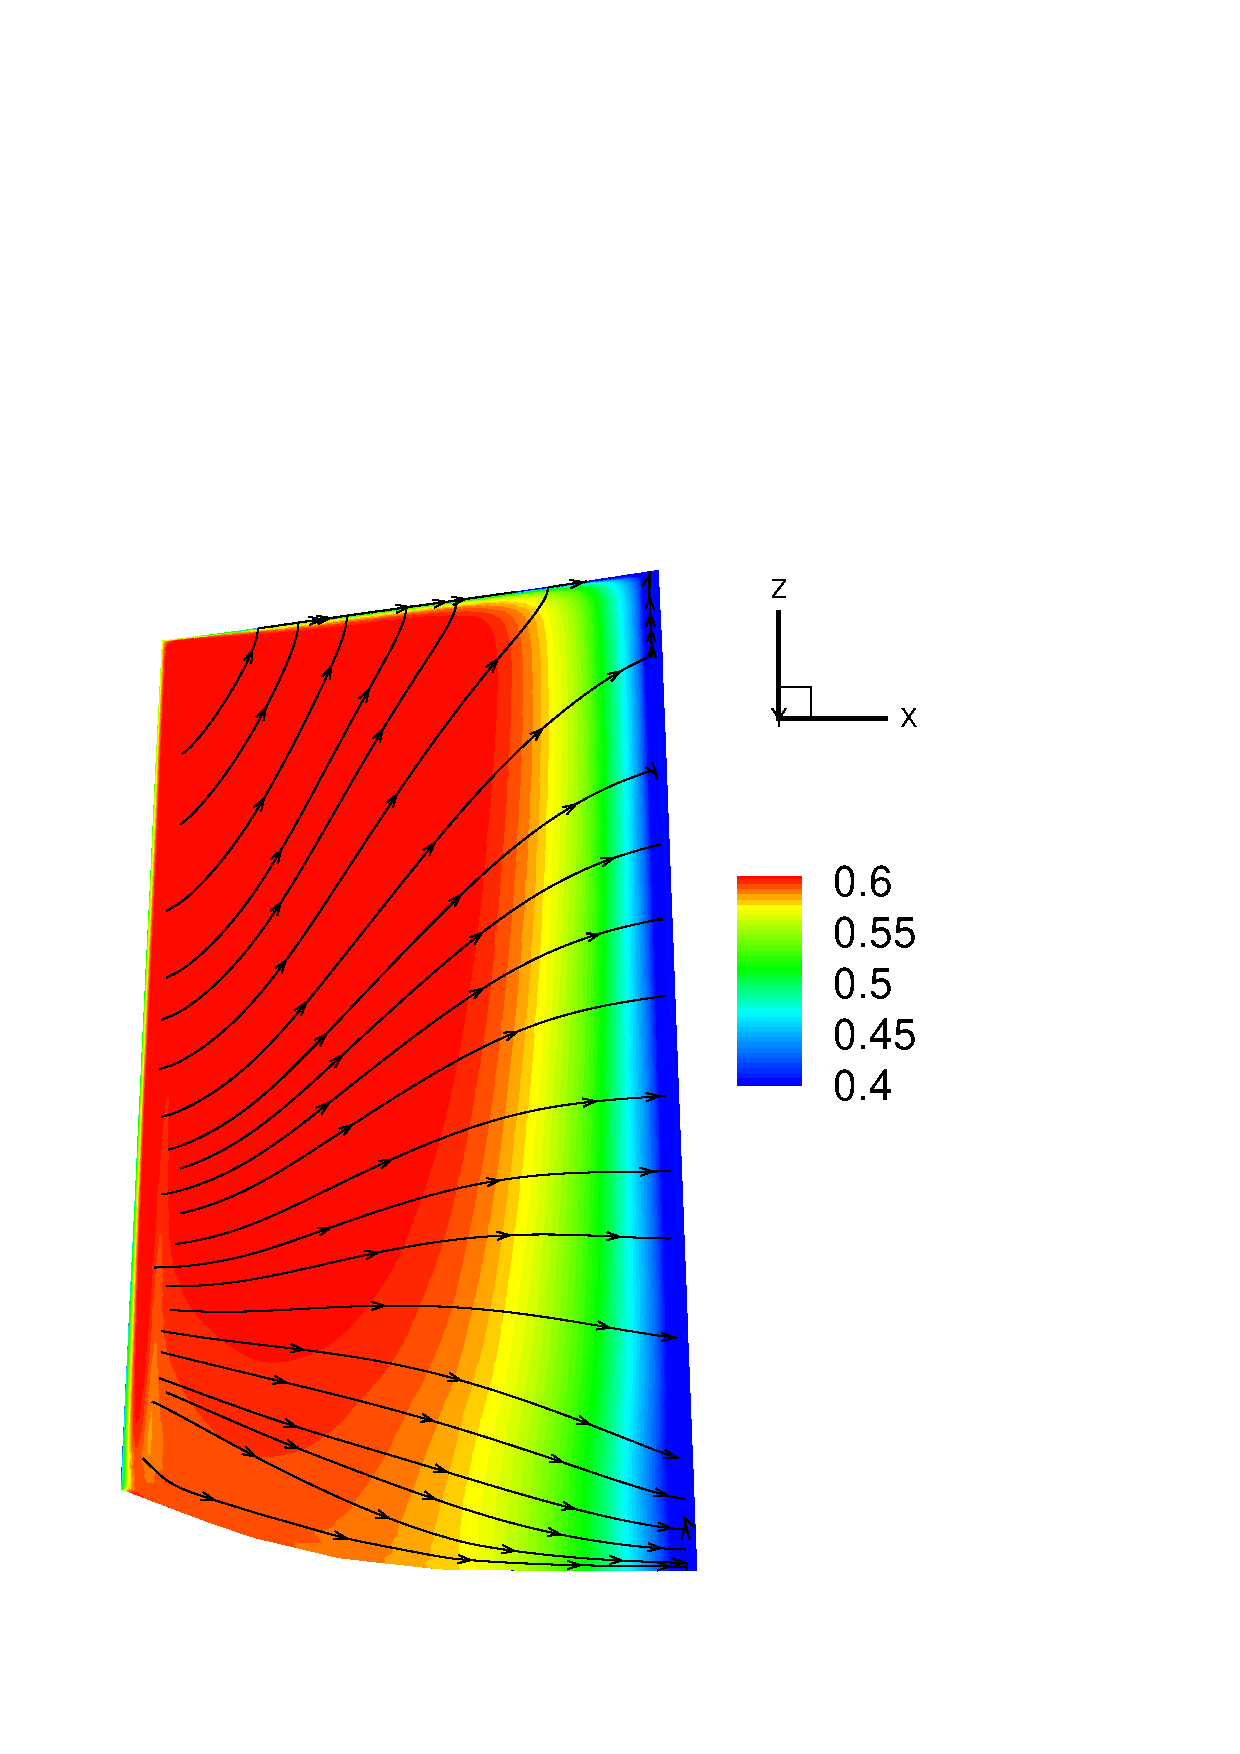
\includegraphics[width=75mm,clip=t]{CHAP_RT27/FIGURE/rotor_traces_pres.pdf}}
        &
    \subfigure[Suction side]
       {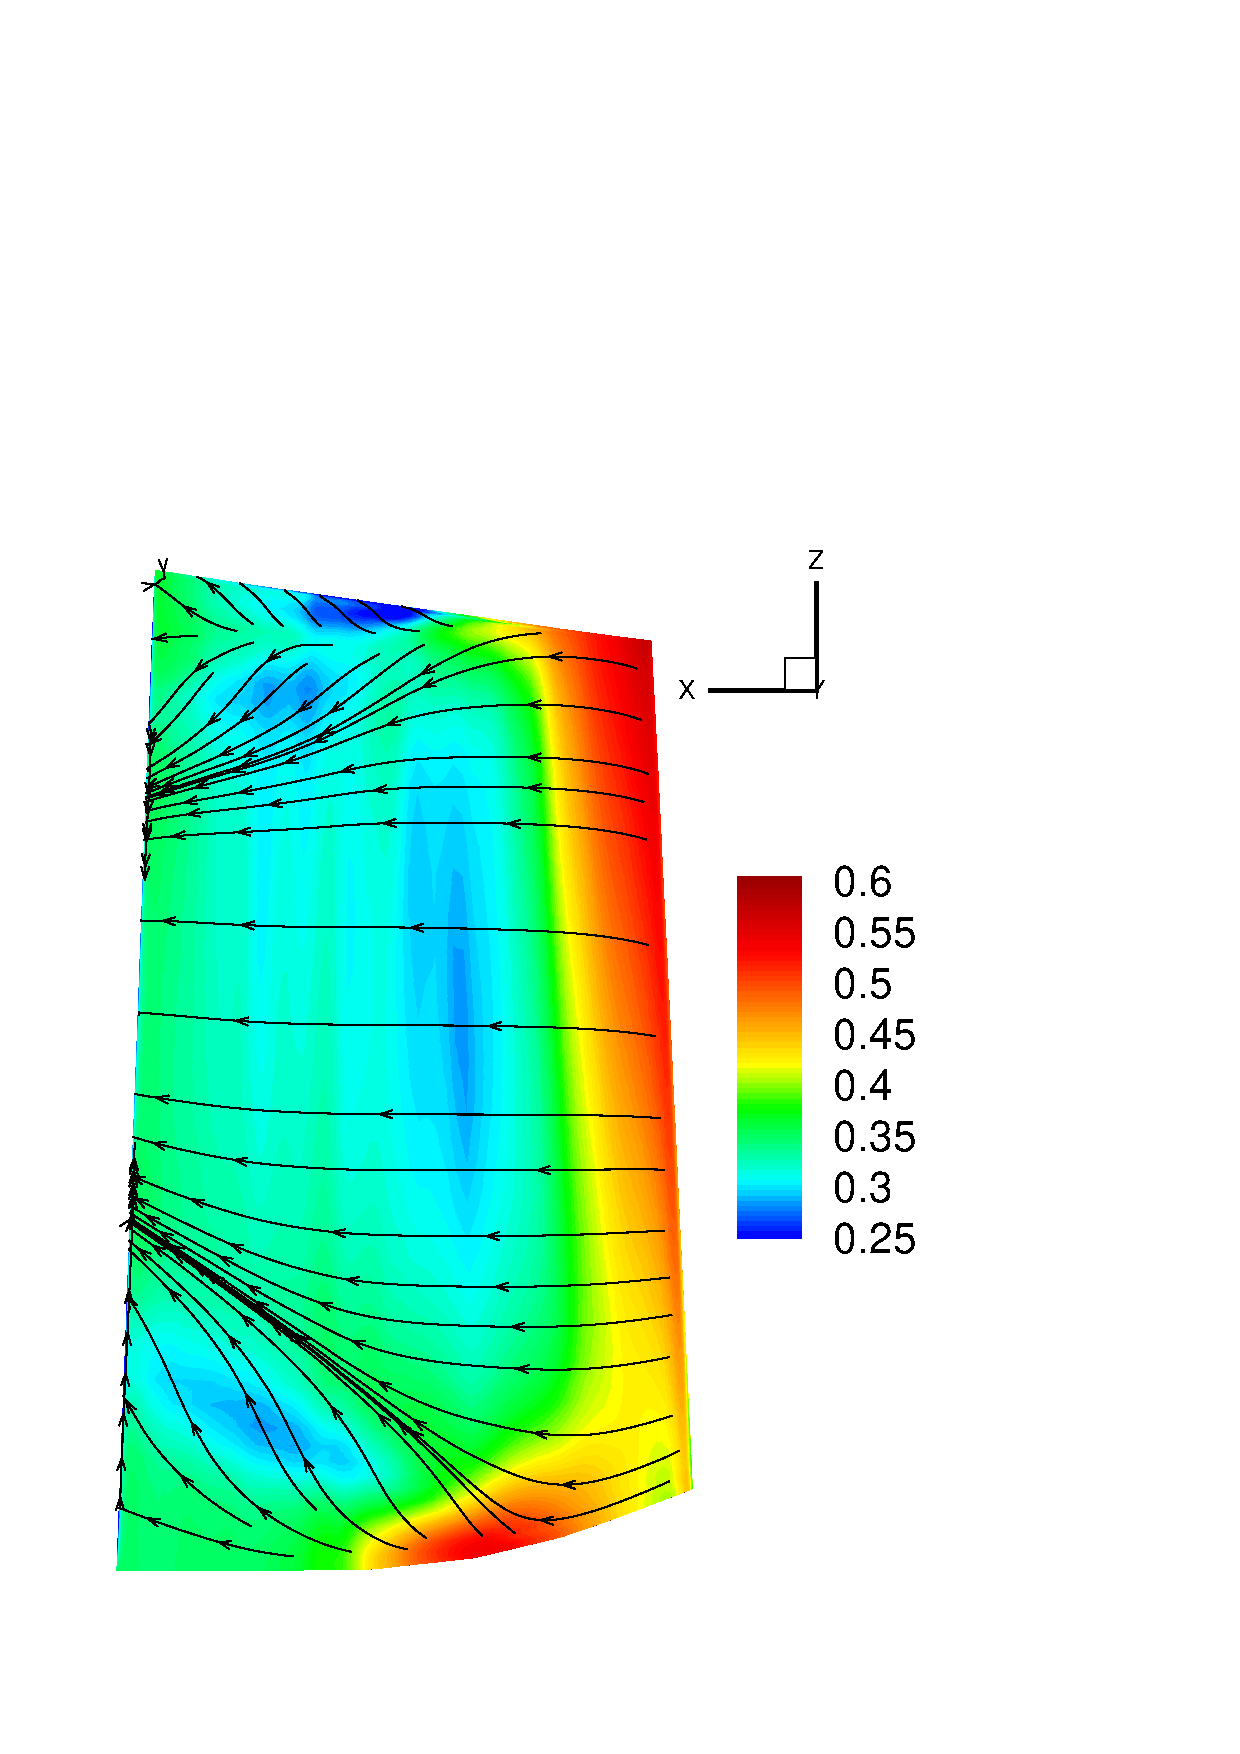
\includegraphics[width=75mm,clip=t]{CHAP_RT27/FIGURE/rotor_traces_suct.pdf}}
  \end{tabular}
 \end{center}
 \vspace{-6mm}
 \caption{Steady state pressure contours $\frac{p}{p\sm{01}}$
          and particle traces on the RT27a rotor surface}
 \label{rotor_blade_traces.fig}
\end{figure}
%
 Fig. \ref{rotor_blade_traces.fig} shows the computed steady state static
 pressure on the rotor blade surface together with particle traces.
 The pressure distribution on the pressure surface is, in the main,
 2D even though the particle traces
 show a significant radial component, especially towards the tip region
 where the tip-clearance pressure jump tends to drive the flow from the pressure
 side towards the suction side of the blade.
 The 3D effects are much more evident from the suction
 surface (Fig. \ref{rotor_blade_traces.fig}b). The flow behaves in a
 2D way only in the middle section, while
 secondary flow effects are very much evident towards both end walls.
 In particular, the separation line caused by the suction side
 leg of the horseshoe vortex is clearly visible at the hub end wall.
 The migration of the separation line
 towards mid-section is caused by the rotation of the passage vortex.
 Such a separation line is also present at the tip end wall but
 the flow pattern is more complicated.
 This is caused by the interaction of the passage and tip-leakage
 vortices which result in counter-rotating flow structures.
 Section \ref{rt27_secondaryflow.subsec} will present a more detailed
 discussion of these secondary flow effects.

 Fig. \ref{rotor_blade_machis1.fig} shows a comparison of predicted and measured
 isentropic Mach number blade distributions at mid-height section.
%
\begin{figure}
  \centerline{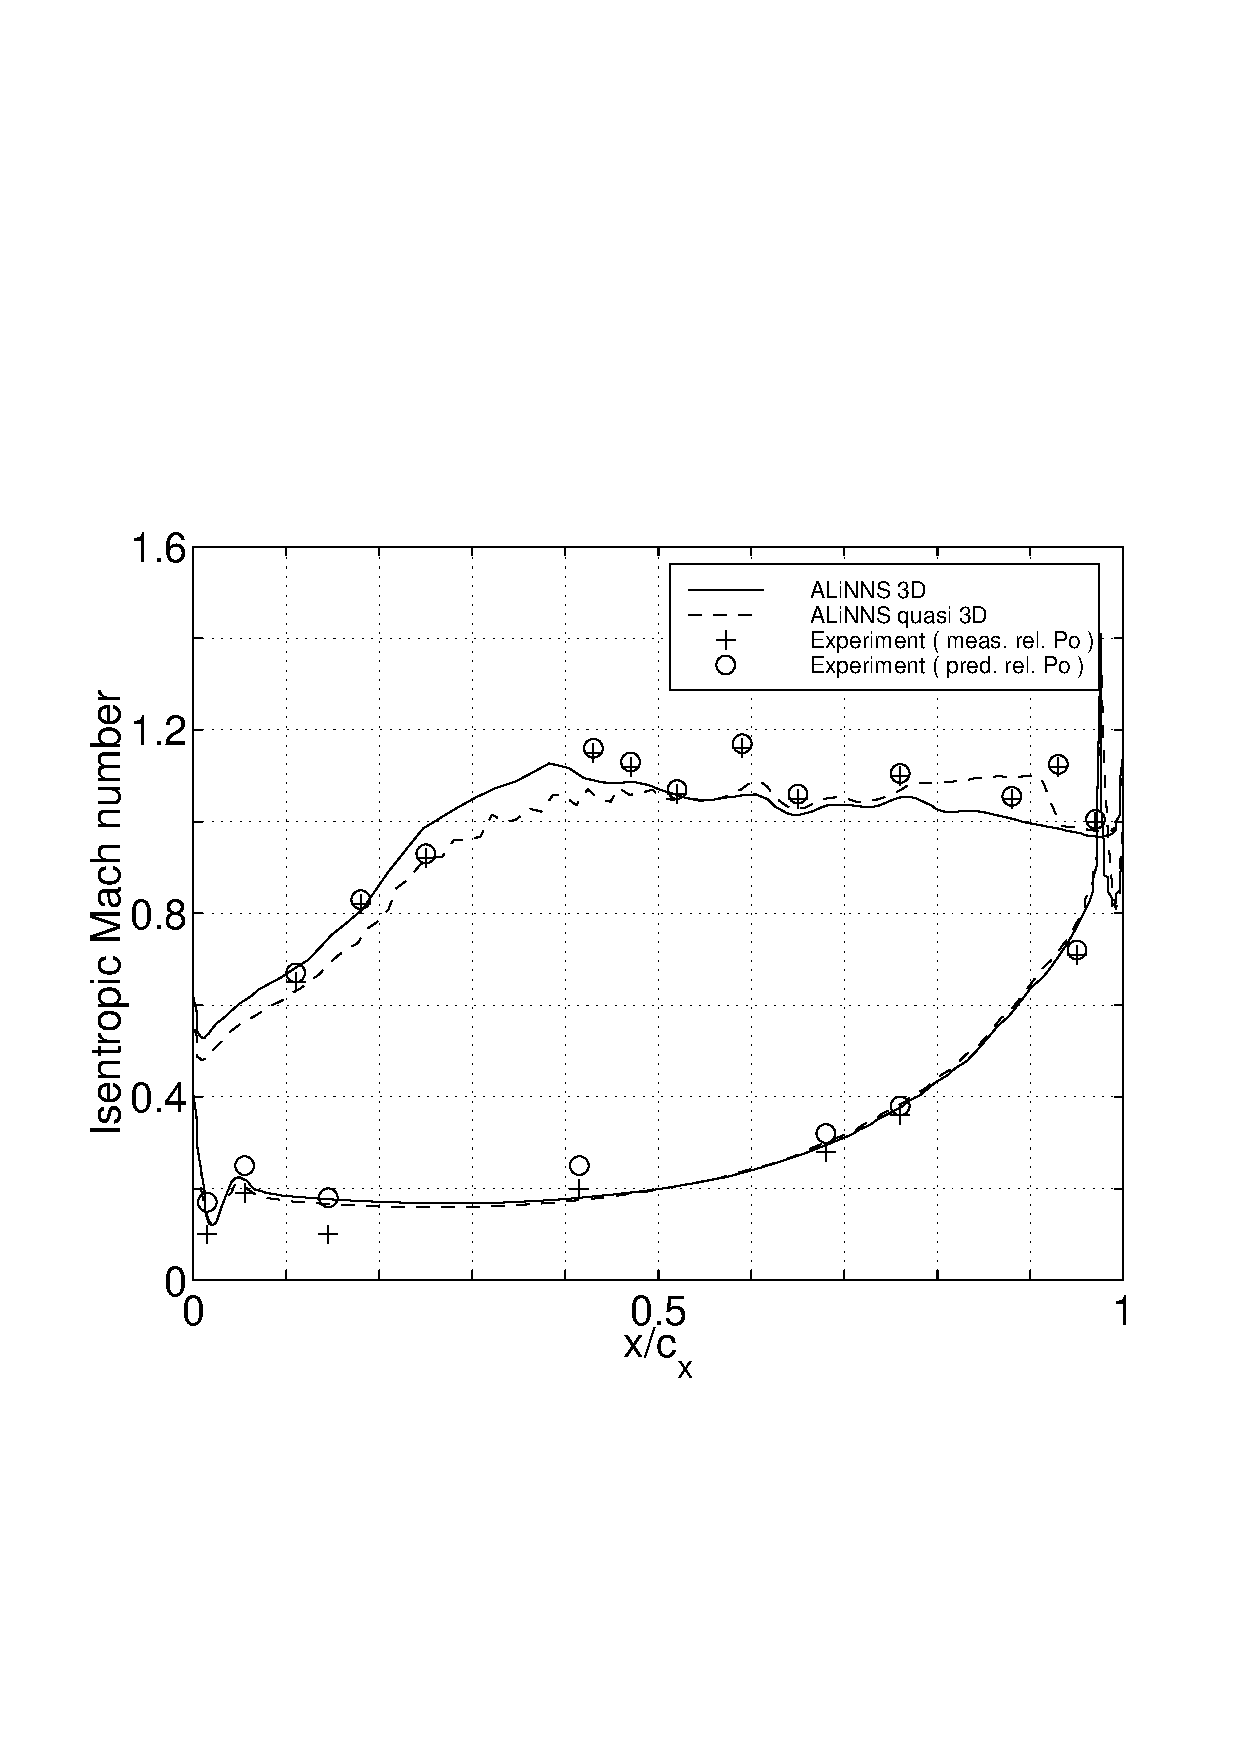
\includegraphics[width=100mm,clip=t]{CHAP_RT27/FIGURE/mid.pdf}}
  \caption{Isentropic steady-state Mach number distribution at
           mid-height section of RT27a rotor blade}
  \label{rotor_blade_machis1.fig}
\end{figure}
%
 The two experimental Mach number distributions are calculated from
 the time-mean unsteady static pressures but using two different values of
 the rotor-relative total pressures at the leading-edge: the experimental
 and the computed values.
 The discrepancy between the two measured curves can be considered to
 be an indicator of the experimental sensitivity to the rotor relative inlet
 total pressure.
 Fig. \ref{rotor_le.fig} shows the comparison between the measured and computed
 leading-edge pressure values along the radial direction.
 In addition to the distribution obtained from the 3D
 steady-state computation,
 Fig. \ref{rotor_blade_machis1.fig} reports the result of a quasi-3D
 calculation performed at mid-height section.
 The true 3D result agrees, with the measurements,
 better in the forward part
 of the blade suction surface while it overestimates the
 exit pressure.
%
\begin{figure}
  \centerline{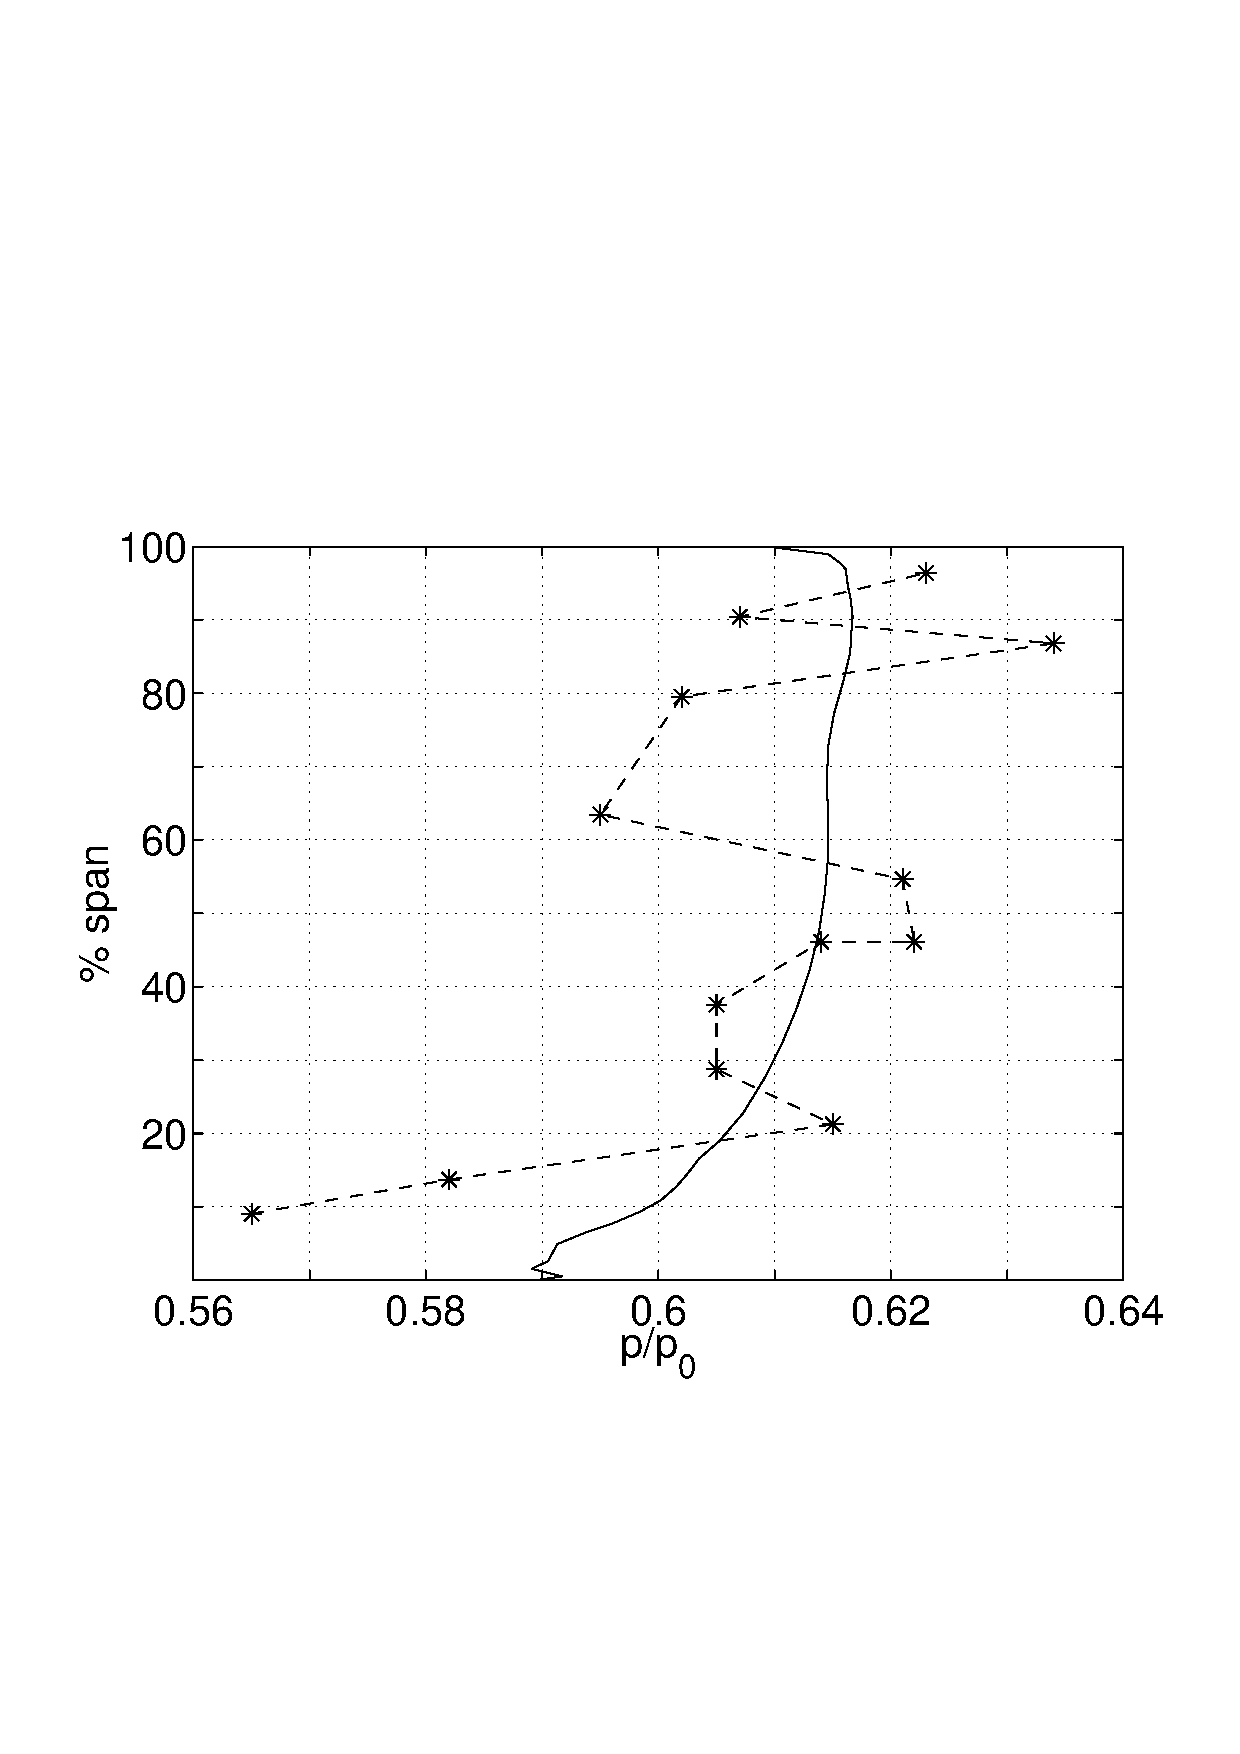
\includegraphics[width=100mm,clip=t]{CHAP_RT27/FIGURE/rot_le.pdf}}
  \caption{RT27a rotor leading-edge pressure levels. (*) Leading-edge kulite
           measured data, (-) computed}
  \label{rotor_le.fig}
\end{figure}
%
 Fig. \ref{rotor_blade_machis2.fig} shows a comparison of the predicted
 isentropic Mach number blade distributions at 5, 10, 90 and 95\%
 spans with the time-averaged measured data.
 The overall agreement is reasonably good although some discrepancies
 are worth mentioning.
 As for the mid-height blade distribution of Fig. \ref{rotor_blade_machis1.fig},
 the computed results in the trailing-edge region of the suction surface
 underestimate the measured isentropic Mach number.
 The reasons for such discrepancies are not entirely clear. However, it should
 be noted that experimental data represent averaged unsteady flow which,
 under certain circumstances may be different from the true steady flow.
 This is probably the case of regions where shock waves are present, i.e.
 towards the trailing-edge region of the suction surface.
%
%
\begin{figure}[ht]
 \begin{center}
  \begin{tabular}{cc}
    \subfigure[Root section]
       {\hspace{-10mm}\includegraphics[width=75mm,clip=t]{CHAP_RT27/FIGURE/hub.pdf}}
        &
    \subfigure[Mid-root section]
       {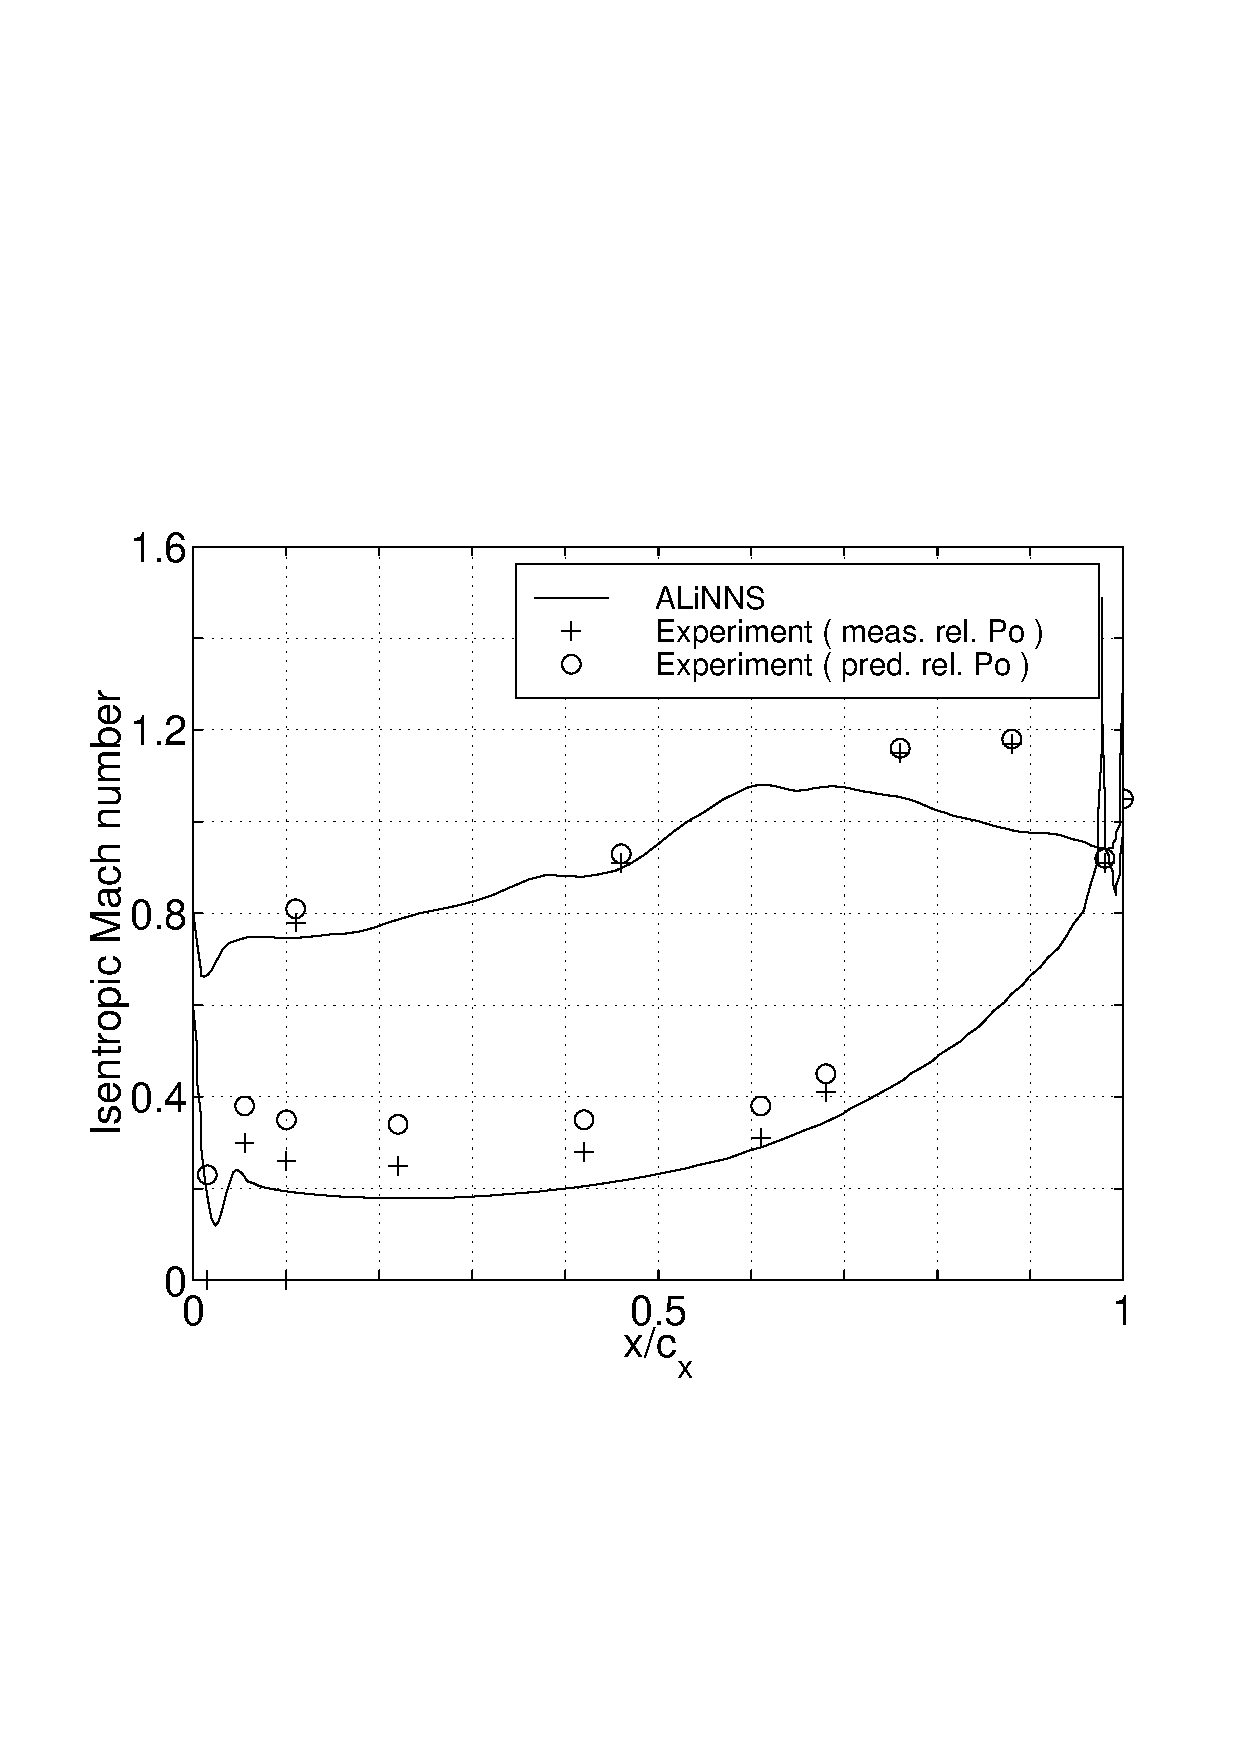
\includegraphics[width=75mm,clip=t]{CHAP_RT27/FIGURE/midhub.pdf}}
       \vspace{-4mm}\\
    \subfigure[Mid-tip section]
       {\hspace{-10mm}\includegraphics[width=75mm,clip=t]{CHAP_RT27/FIGURE/midtip.pdf}}
        &
    \subfigure[Tip section]
       {\includegraphics[width=75mm,clip=t]{CHAP_RT27/FIGURE/tip.pdf}}
  \end{tabular}
 \end{center}
 \vspace{-8mm}
 \caption{RT27a rotor blade: isentropic steady-state Mach number distribution
          at different span-wise positions}
 \label{rotor_blade_machis2.fig}
\end{figure}
%

 One feature that is common to Figs. \ref{rotor_blade_machis1.fig}
 and \ref{rotor_blade_machis2.fig} is that the pressure-side isentropic
 Mach number distribution is almost the same for all span-wise
 positions, a feature that is also evident from Fig. \ref{rotor_blade_traces.fig}a.
 The suction-side results show considerable deviations from the base 2D flow
 due to secondary and tip-leakage flows effects.
 Fig. \ref{rotor_blade_machis2.fig}a shows that forward position of
 the suction side is unloaded relative to midspan values.
 At mid-root, the unloading in the forward position is less pronounced
 and the results are closer to the midspan values.
 This trend of a increasing load on the forward position continues all the way
 to the tip.
%
%
%
%
%
\subsection{Secondary and tip-clearance flow}
\label{rt27_secondaryflow.subsec}
%
 Three main vortices were identified in the rotor blade passage:
 the {\em horseshoe} vortex, the {\em passage} vortex and the
 {\em tip-leakage} vortex.
 The formation of first two vortices is connected to the presence
 of velocity gradients near the end wall boundary layers while
 the tip-leakage vortex is caused by the fast moving flow in the gap region.

 The horseshoe vortex has two legs, namely the suction and pressure side legs.
 This vortex is formed around the leading-edge of the blade at the end wall
 regions, in the same way as around any blunt body with its axis
 perpendicular to the wall. The high energy fluid, at the edge
 of the end wall boundary layer, flows away from the leading-edge
 stagnation point, not only around the blade, but also downwards because of
 the lower energy of the fluid below.
 When this high energy fluid reaches the end wall, it flows upstream forming
 a saddle point where the upstream flow separates form the surface.
 Fig. \ref{rotor_hub_traces.fig} shows the static pressure contours as well
 as the particle traces at $1\%$ span. The two separation lines
 caused by the pressure and the suction leg of the horseshoe vortex can
 be seen clearly.
 The suction side leg remains close to the blade and then, as indicated in
 Fig. \ref{rotor_blade_traces.fig}, travels up the suction surface,
 while the pressure side leg crosses the blade passage to the suction
 side of the other blade.
%
\begin{figure}
 \centerline{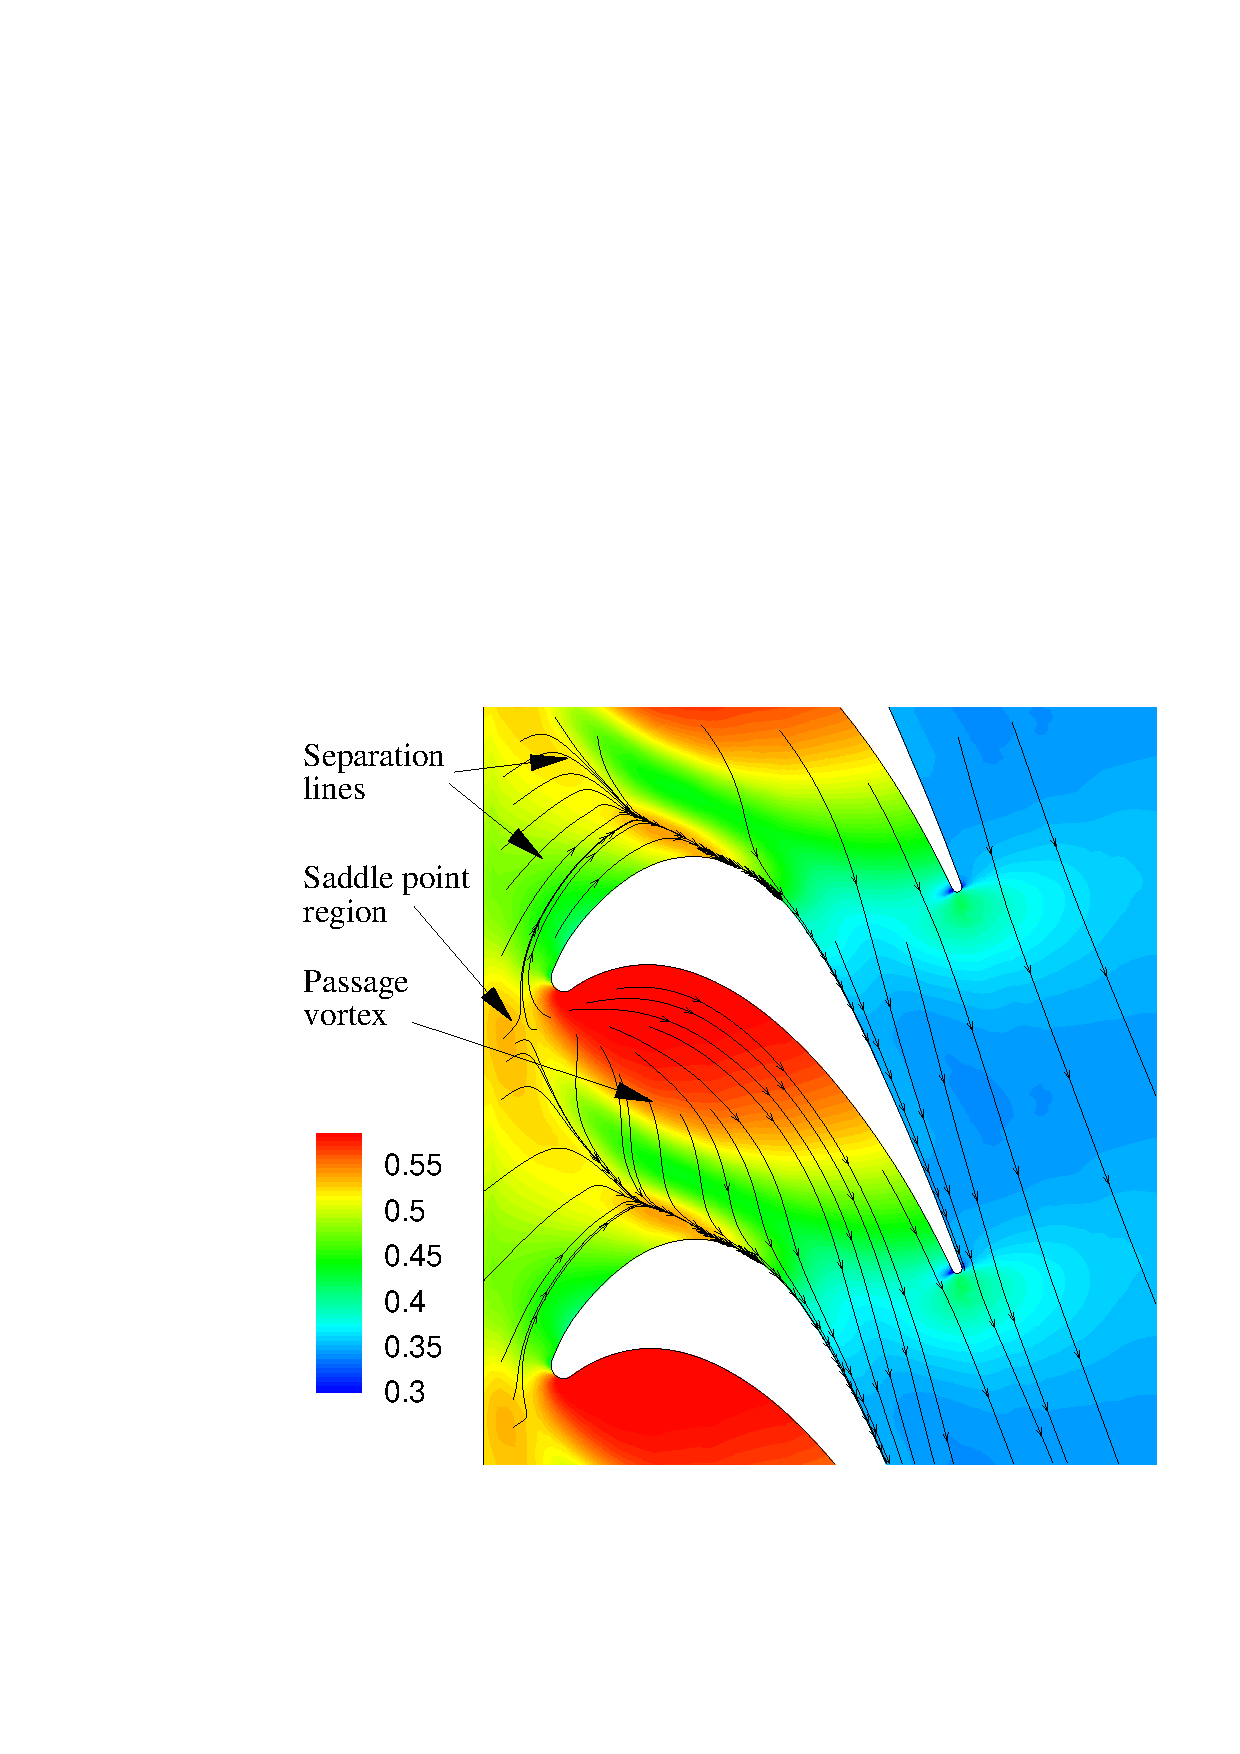
\includegraphics[width=100mm]{CHAP_RT27/FIGURE/rotor_hub_traces.pdf}}
 \caption{Steady state pressure contours $\frac{p}{p\sm{01}}$
          and particle traces at $1\%$ span of RT27a rotor blade}
 \label{rotor_hub_traces.fig}
\end{figure}
%
 The detail is very complex, but the same main features were noted
 by other researchers (Sieverding \citeyearNP{Sieverding:1},
 Gregory-Smith \citeyearNP{Gregory:1}).

 The passage vortex is associated with the turning
 of the vorticity vector, and its main effect occurs in the middle of
 the passage. Its rotation is in the same sense as the pressure side leg
 of the horseshoe vortex and the two evolve and merge together.
 Fig. \ref{rotor_passage_traces.fig} shows the particle traces at two
 consecutive axial planes. At an axial plane $15\%$ chord downstream
 of the leading-edge, a recirculating flow pattern,
 formed by the passage vortex and pressure side leg of the
 horseshoe vortex, is centered in the middle of the passage.
 Within the blade passage the vortex is convected by its own flow field
 from the pressure surface towards the suction surface as indicated
 in Fig. \ref{rotor_passage_traces.fig}b.
%
%
%
\begin{figure}[ht]
 \begin{center}
  \begin{tabular}{lll}
    \hspace{-10mm}
    \subfigure[$15\%$ axial chord]
       {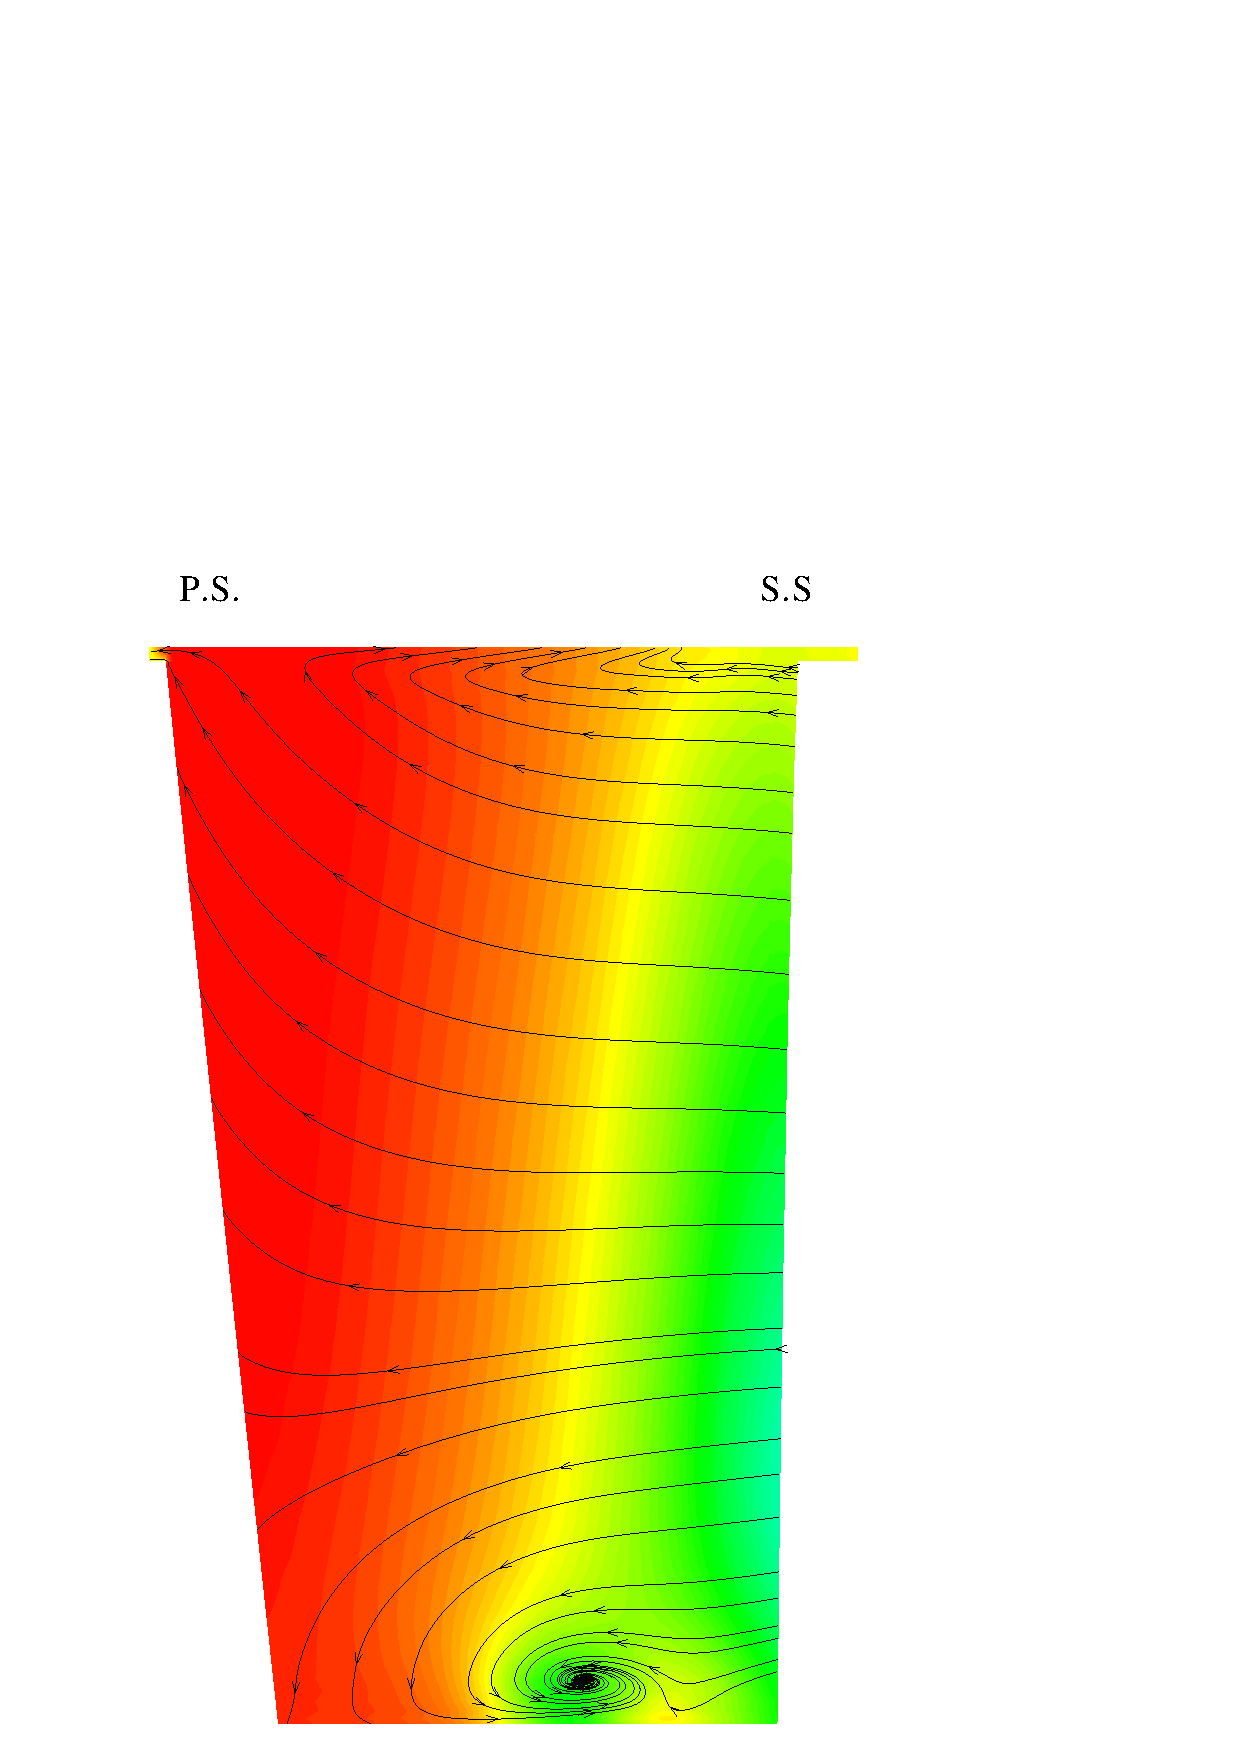
\includegraphics[width=60mm,clip=t]{CHAP_RT27/FIGURE/slid056.pdf}}
        &
    \subfigure[$30\%$ axial chord]
       {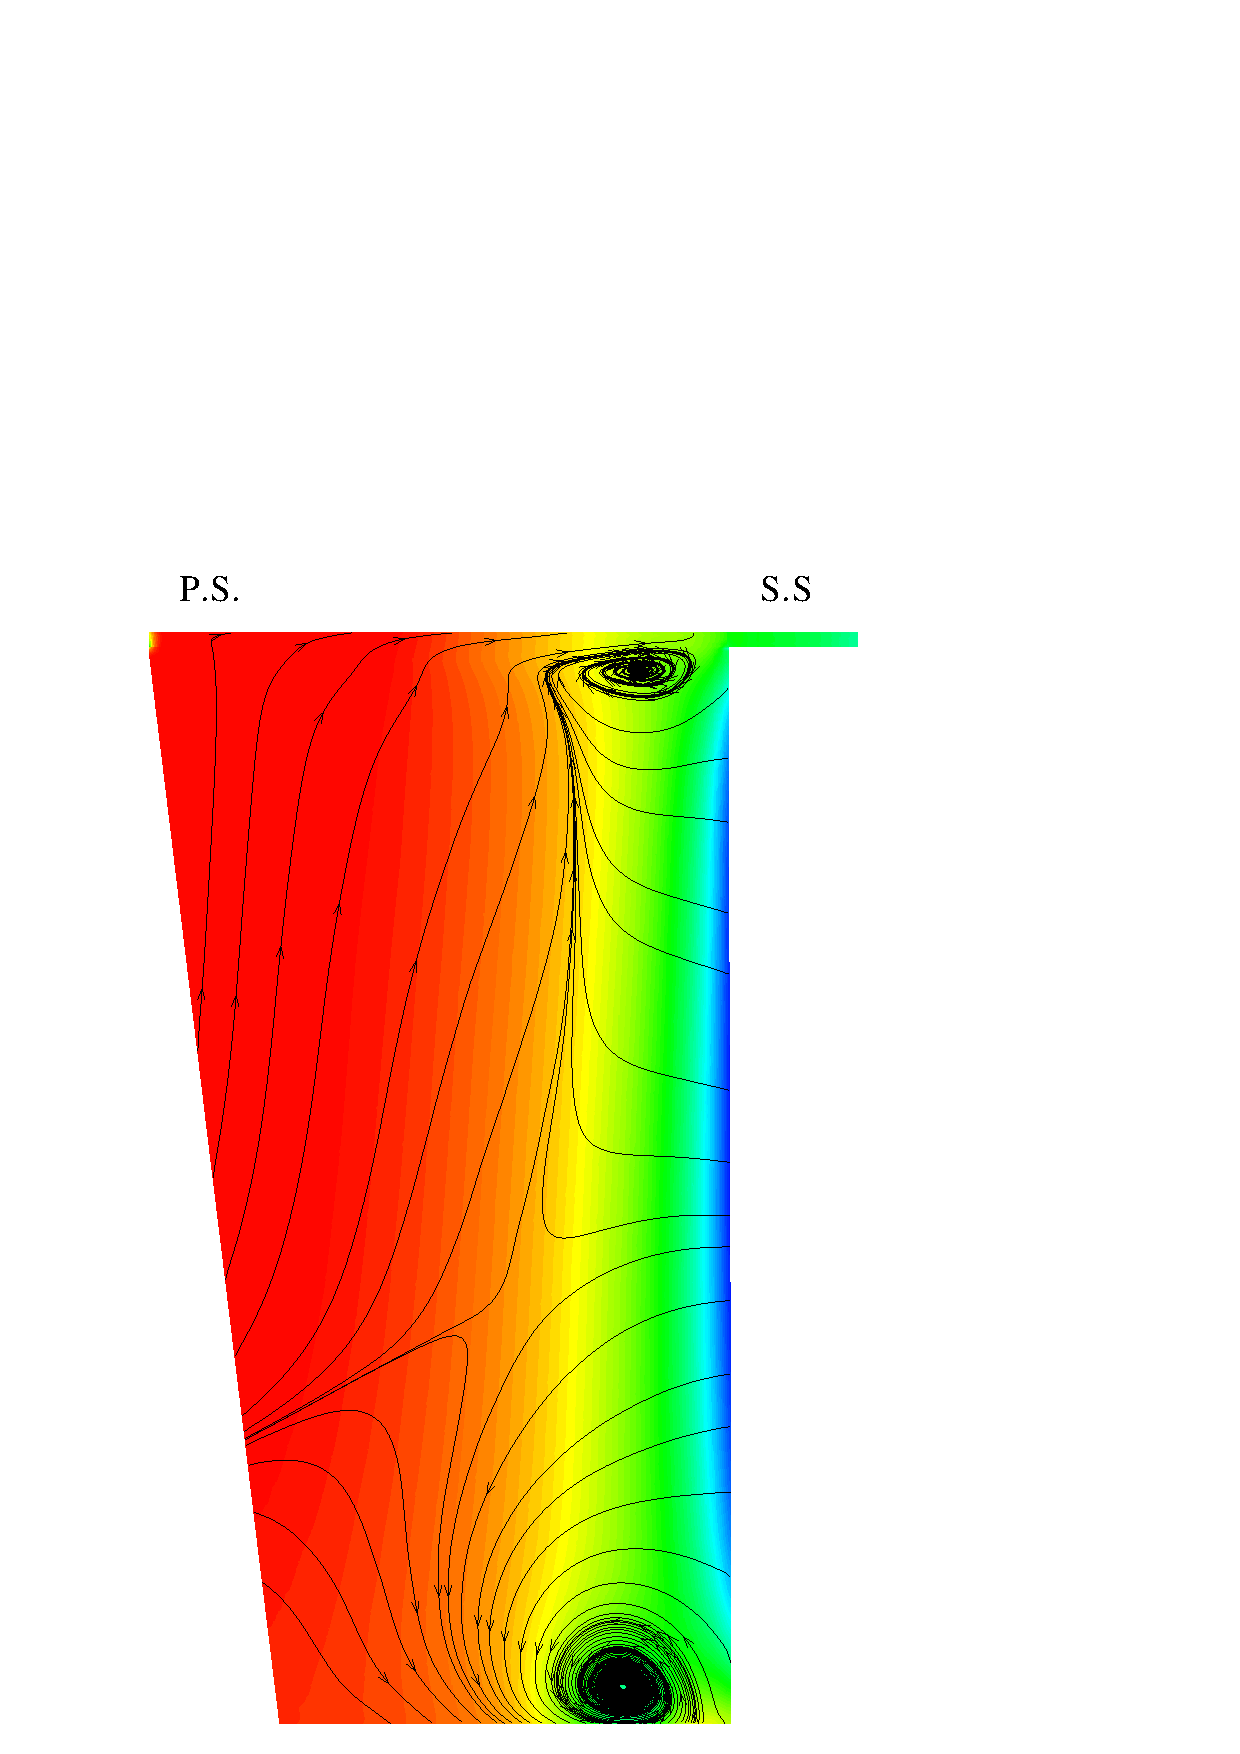
\includegraphics[width=60mm,clip=t]{CHAP_RT27/FIGURE/slid060.pdf}}
        &
    \subfigure
       {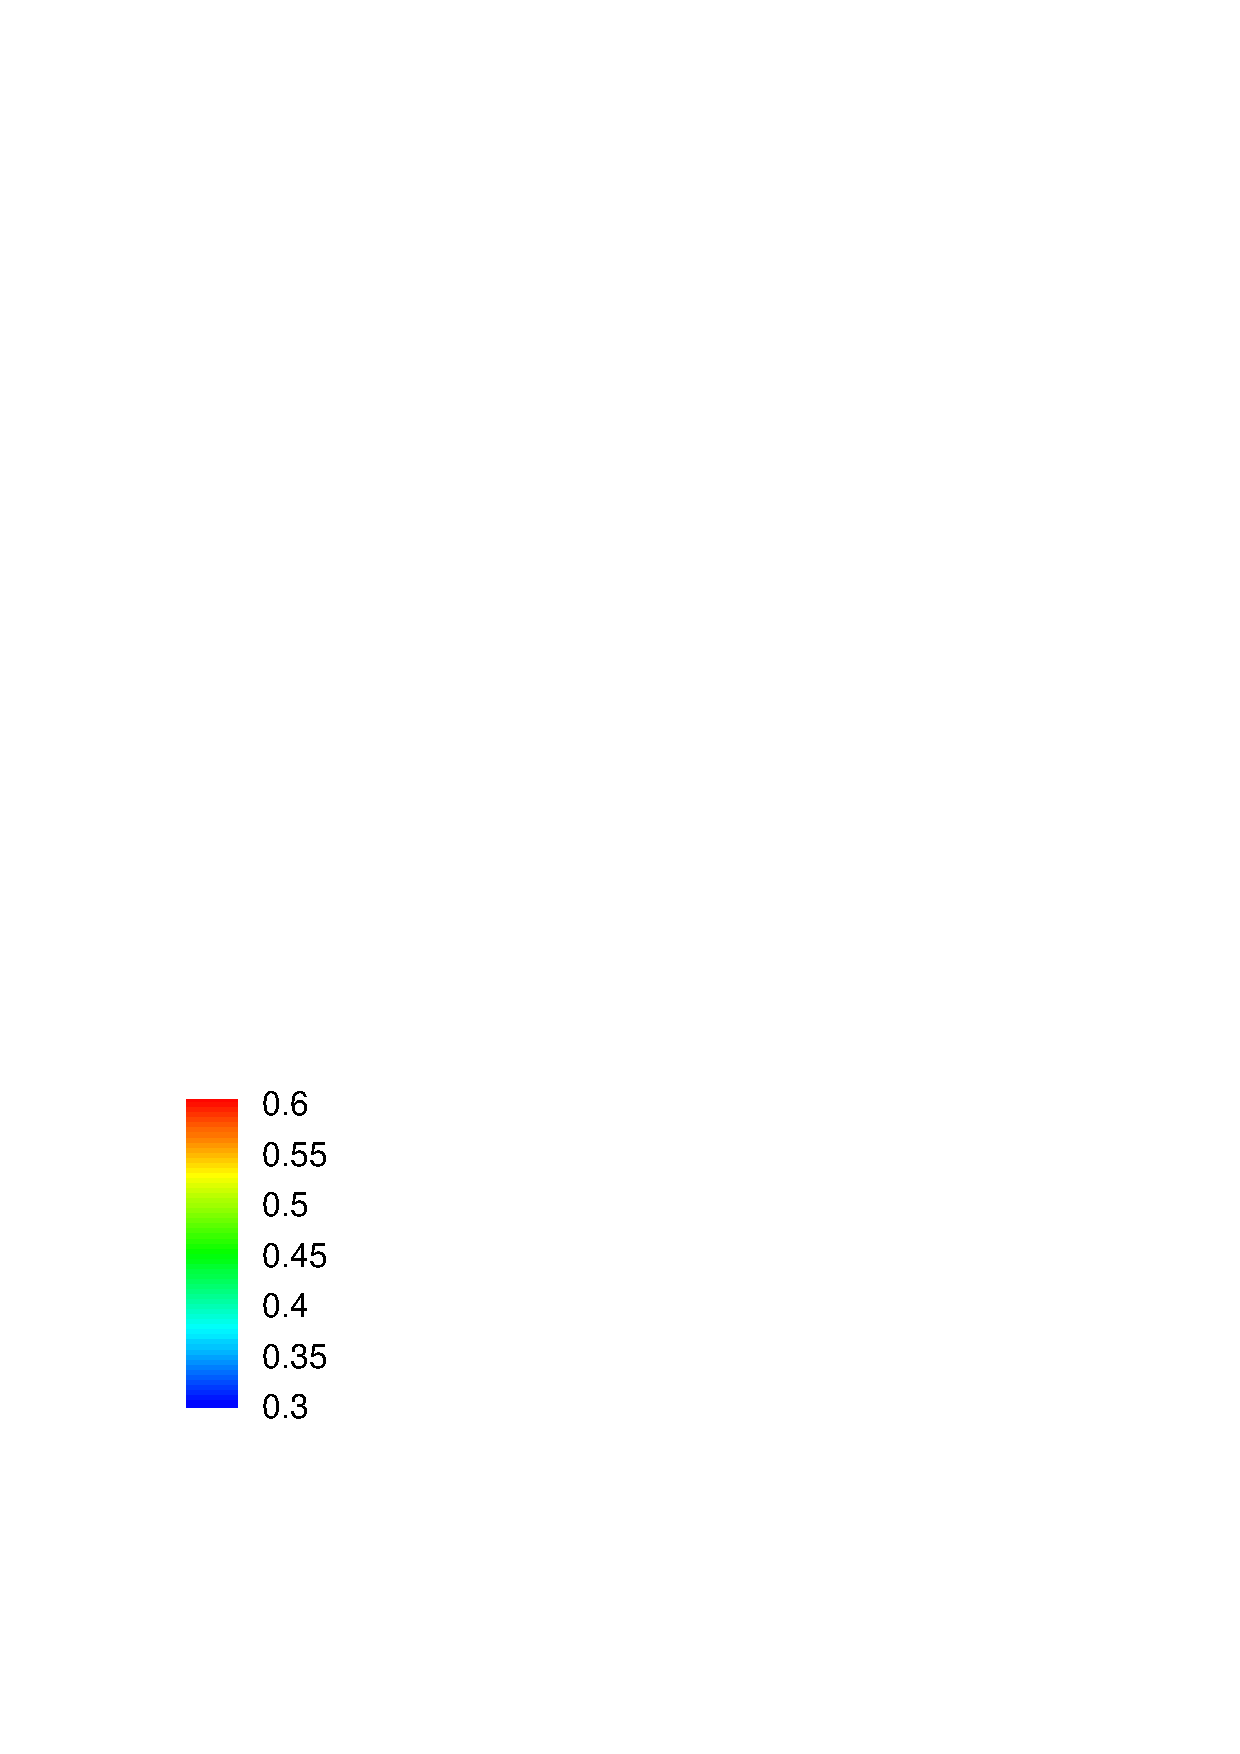
\includegraphics[width=20mm,clip=t]{CHAP_RT27/FIGURE/slid0pr.pdf}}
  \end{tabular}
 \end{center}
 \vspace{-8mm}
 \caption{Pressure contours $\frac{p}{p\sm{01}}$ and particle traces
          at different $r\theta-r$ planes in the RT27a rotor passage}
 \label{rotor_passage_traces.fig}
\end{figure}
%
 The formation of the passage vortex is a natural consequence
 of the interaction between the shear flow at the end wall and
 the turning of the blade.
 The mainstream flow sets up a pressure gradient across the blade
 passage, from the suction to the pressure surfaces, which
 can be approximated by the following relationship:

%
\beq
  \fpd{p}{r} = \frac{\rho u\sm{r}\se{2}}{r}
  \label{equil_radial.eq}
\eeq
%
 where $r$ is the local radius of the turning of the flow caused
 by the blade passage.
 The slower moving boundary layer fluid is subjected to this same
 pressure gradients, but since the velocity $u\sm{r}$ in the boundary layer is
 smaller than the mainstream one, the radius of curvature $r$
 must be smaller.
 Thus in a 3D blade row, the flow on the end wall is
 directed from pressure to suction surface as shown in Fig. \ref{rotor_hub_traces.fig},
 and to preserve continuity, there is a back flow further away from the
 end wall, leading to the vortical flow shown in
 Fig. \ref{rotor_passage_traces.fig}.

 ~\newline
 The flow at the tip is somewhat more complicated. The orifice formed by the
 tip gap experiences essentially the same pressure difference as that
 across the blade.
 Fig. \ref{rotor_tip_traces.fig} shows the static pressure contours as well as
 the particle traces for a radial section inside the tip-gap.
%
\begin{figure}
 \centerline{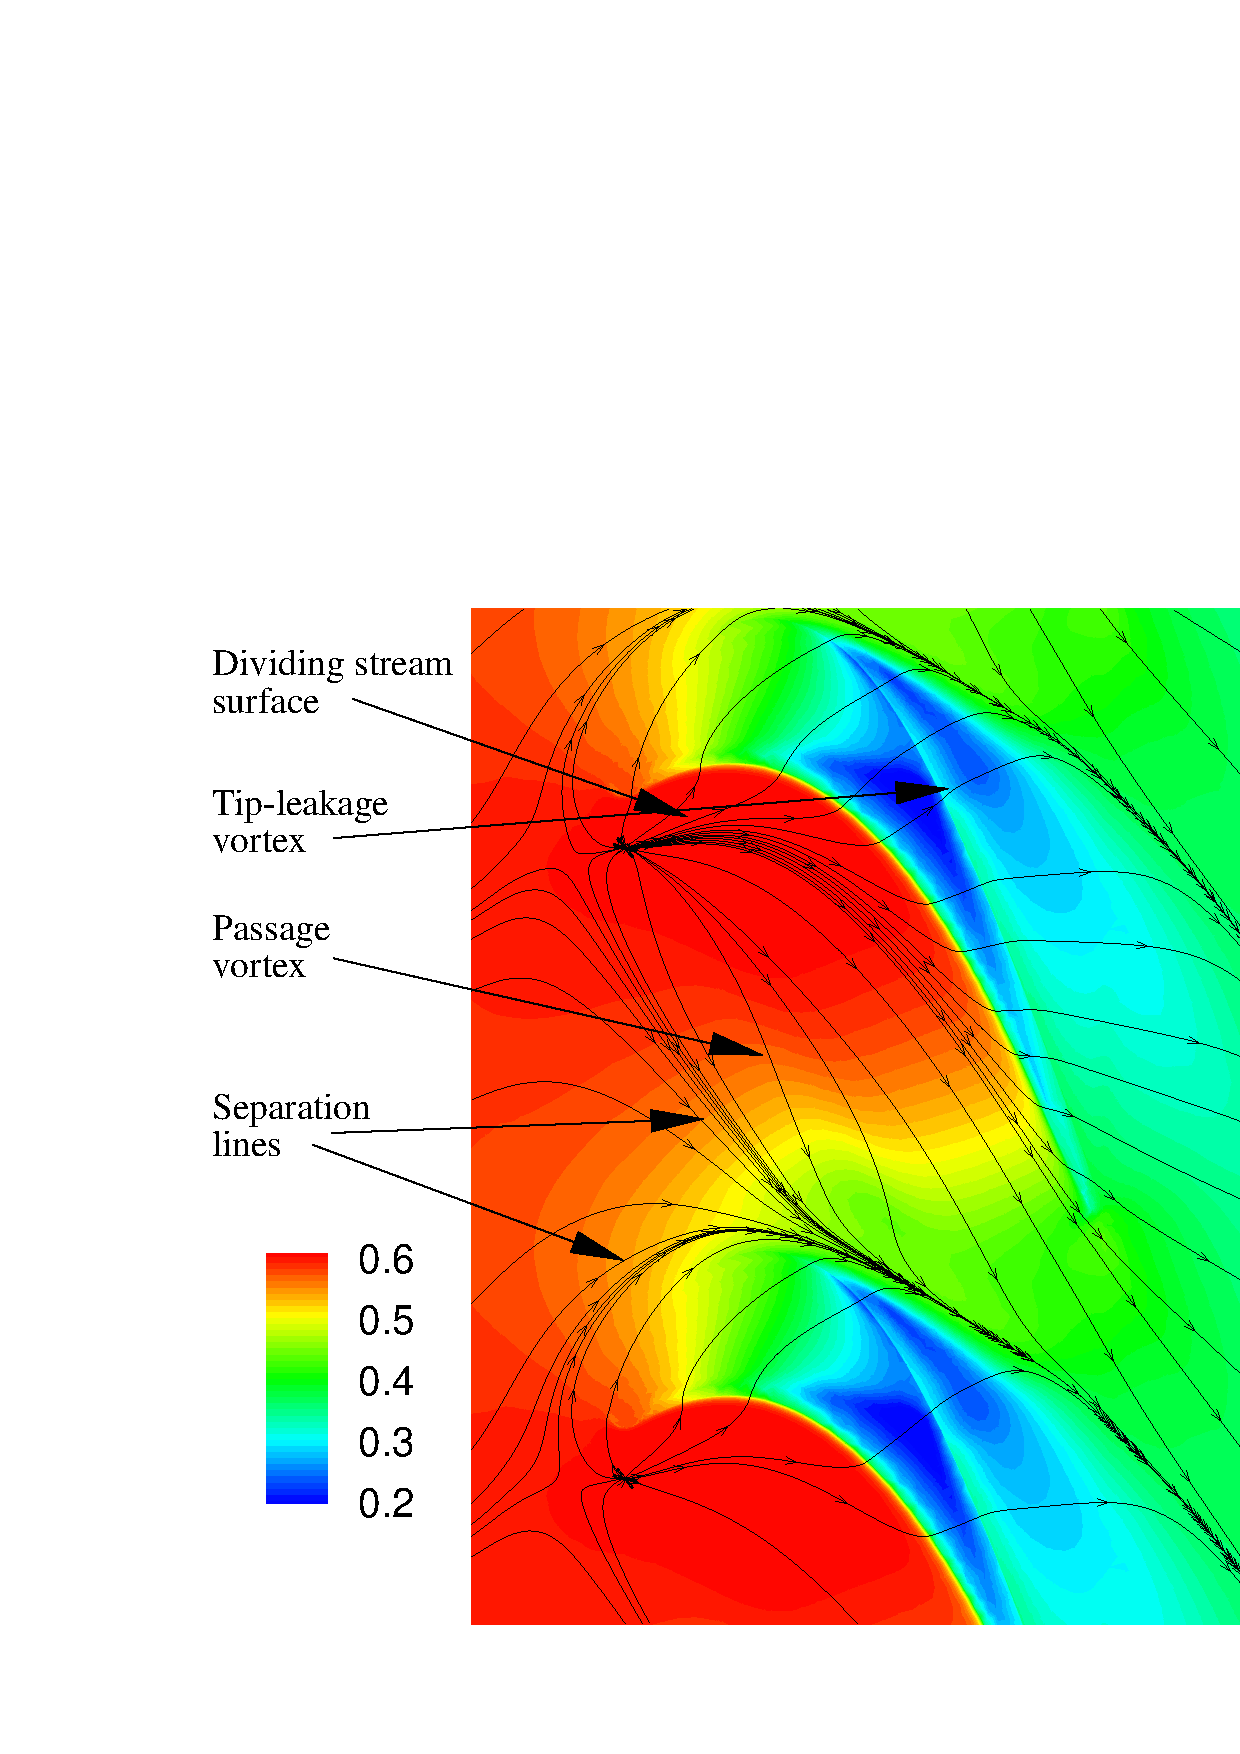
\includegraphics[width=100mm]{CHAP_RT27/FIGURE/rotor_tip_traces.pdf}}
 \caption{Steady state pressure contours $\frac{p}{p\sm{01}}$
          and particle traces inside the RT27a rotor tip-gap region}
 \label{rotor_tip_traces.fig}
\end{figure}
%
 This pressure ratio across the gap accelerates the flow up to supersonic
 conditions. The clearance flow then emerges from the gap with very high velocity
 at an oblique angle relative to the passage flow. The resulting strong interaction
 with the passage flow, including the developing passage vortex of
 Fig. \ref{rotor_tip_traces.fig}, causes the leakage flow to roll up into a vortex
 known as tip-leakage vortex. Such a vortex results in a structure which has a
 vorticity in direction to that of the passage vortex.
 Yamamoto \citeyear{Yamamoto:1} investigated the interaction mechanism
 between tip leakage flow and the passage vortex in some detail.
 At the trailing-edge, the leakage flow pushes the passage vortex away from
 the suction surface, a feature that is evident from Fig. \ref{rotor_tip_traces.fig}.
 Also Yamamoto \citeyear{Yamamoto:1} suggests that the interaction between the
 two vortex structures results in an elongation and distortion of the passage vortex.
 In particular, the leakage flow pushes the secondary flow towards midspan.
 This seems to be in an agreement with what is shown in
 Fig. \ref{rotor_blade_traces.fig}.

 Another important feature of the tip-clearance flow
 is the formation of a dividing stream surface between the fluid which is swept
 into the gap and that which is driven across the passage in the usual way.
 Such a stream surface is evident in Fig. \ref{rotor_tip_traces.fig}
 where it lies at about one fifth of the blade pitch from the pressure
 surface. The exact position of the division stream surface is a function
 of the clearance and probably other parameters such as the blade loading
 (Sjolander \& Amrud \citeyearNP{Sjolander:1}).

 Fig. \ref{rotor_tip_traces.fig} also shows the absence of the
 stagnation point due to the presence of the clearance.
 On the other hand, the two separation lines of the horseshoe
 vortex are still present.
 For larger clearances, Sjolander \& Amrud \citeyear{Sjolander:1} show
 that the tip horseshoe vortex disappears.
%
%
%
